\documentclass{article}
\usepackage[top=3cm, bottom=3cm, outer=3cm, inner=3cm]{geometry}
\usepackage{graphicx}
\usepackage{url}
\usepackage{hyperref}
\usepackage{array}
%\usepackage{multicol}
\newcolumntype{x}[1]{>{\centering\arraybackslash\hspace{0pt}}p{#1}}
\usepackage[numbers,super]{natbib}
\usepackage{pdfpages}
\usepackage{multirow}
\usepackage{cite}
\usepackage[normalem]{ulem}
% %% Own Packages %%
% \usepackage{csquotes}
% \MakeOuterQuote{"}
\usepackage{listings}
\usepackage{float}
\usepackage[shortlabels]{enumitem}



%%%%%%%%%%%%%%%%%%%%%%%%%%%%%%%%%%%%%%%%%%%%%%%%%%%%%%%%%%%%%%%%%%%%%%%%%%%%
%%%%%%%%%%%%%%%%%%%%%%%%%%%%%%%%%%%%%%%%%%%%%%%%%%%%%%%%%%%%%%%%%%%%%%%%%%%%
\newcommand{\csemail}{vmachacaa@ulasalle.edu.pe}
\newcommand{\csdocente}{MSc. Vicente Enrique Machaca Arceda}
\newcommand{\cscurso}{Construcción De Software}
\newcommand{\csuniversidad}{Universidad La Salle}
\newcommand{\csescuela}{Escuela Profesional de Ingeniería de Software}
\newcommand{\cspracnr}{04}
\newcommand{\cstema}{Base de datos}
%%%%%%%%%%%%%%%%%%%%%%%%%%%%%%%%%%%%%%%%%%%%%%%%%%%%%%%%%%%%%%%%%%%%%%%%%%%%
%%%%%%%%%%%%%%%%%%%%%%%%%%%%%%%%%%%%%%%%%%%%%%%%%%%%%%%%%%%%%%%%%%%%%%%%%%%%


\usepackage[english,spanish]{babel}
\usepackage[utf8]{inputenc}
\AtBeginDocument{\selectlanguage{spanish}}
\renewcommand{\figurename}{Figura}
\renewcommand{\refname}{Referencias}
\renewcommand{\tablename}{Tabla} %esto no funciona cuando se usa babel
\AtBeginDocument{%
	\renewcommand\tablename{Tabla}
}

\usepackage{fancyhdr}
\pagestyle{fancy}
\fancyhf{}
\setlength{\headheight}{30pt}
\renewcommand{\headrulewidth}{1pt}
\renewcommand{\footrulewidth}{1pt}
\fancyhead[L]{\raisebox{-0.2\height}{
\includegraphics[width=4cm]{.././img/lasalle_black.pdf}}}
\fancyhead[C]{}
\fancyhead[R]{\fontsize{7}{7}\selectfont	\csuniversidad \\ \csescuela \\ \textbf{\cscurso} }
\fancyfoot[L]{MSc. Vicente Machaca}
\fancyfoot[C]{\cscurso}
\fancyfoot[R]{Página \thepage}







\begin{document}

\vspace*{10pt}

\begin{center}
    \fontsize{17}{17} \textbf{ Práctica \cspracnr}
\end{center}
%\centerline{\textbf{\underline{\Large Título: Informe de revisión del estado del arte}}}
%\vspace*{0.5cm}


\begin{table}[H] \centering
    \begin{tabular}{|x{4.7cm}|x{4.8cm}|x{4.8cm}|}
        \hline
        \textbf{DOCENTE} & \textbf{CARRERA} & \textbf{CURSO} \\
        \hline
        \csdocente       & \csescuela       & \cscurso       \\
        \hline
    \end{tabular}
\end{table}


% \begin{table}[H] \centering
%     \begin{tabular}{|x{4.7cm}|x{4.8cm}|x{4.8cm}|}
%         \hline
%         \textbf{PRÁCTICA} & \textbf{TEMA} & \textbf{DURACIÓN} \\
%         \hline
%         \cspracnr         & \cstema       & 2 horas           \\
%         \hline
%     \end{tabular}
% \end{table}


\section{Datos de los estudiantes}
\begin{itemize}
    \item Grupo: 1
    \item Integrantes:
          \begin{itemize}
              \item Elvis Andre Cruces Gomez
              \item Yoshiro Milton Miranda Valdivia
              \item José Alfredo Pinto Villamar
          \end{itemize}
\end{itemize}





\section{Informe}\label{sec:Informe}
\subsection{Problema}
En las escuelas, incluso en las universidades, siempre se ha presentado un
problema para la toma de asistencias y la toma de participaciones de cada
estudiante por curso, sobre todo cuando son aquellos cursos donde hay más de 50
estudiantes matriculados. Esto genera un problema para los profesores incluso
para los estudiantes sobre todo porque a veces no se les escucha o no están
atentos en la toma de asistencia y esto los perjudica ya que se les sube una
inasistencia al sistema. Además, también se pierde demasiado tiempo, ya que al
ser demasiados estudiantes a veces se llega a tomar 30 minutos de la clase ya
que por seguridad los profesores toman la lista 2 veces para evitar confusiones.

\subsection{Objetivos}
Como objetivo principal, planteamos crear una aplicación, que nos permita:
\begin{itemize}
    \item Tomar la asistencia de los estudiantes para cada curso, mediante
    el reconocimiento facial, facilitando el trabajo del profesor y que no
    pierda tiempo, y que los estudiantes al marcar la asistencia sepan que si se
    les marcó y no tengan que preguntar o quedarse con la duda.
    \item Anotar las participaciones de los estudiantes por cada
    intervención asertiva que hagan en los diferentes cursos en los que estén
    matriculados para tener un mejor manejo de la lista de participaciones.
    \item Reducir el tiempo que demora realizar el proceso de toma de
    asistencia y de participaciones por alumno.
\end{itemize}

\subsection{Propuesta}
\subsubsection{Arquitectura}
\pagebreak %% fixed
\begin{figure}[h]
    \centering
    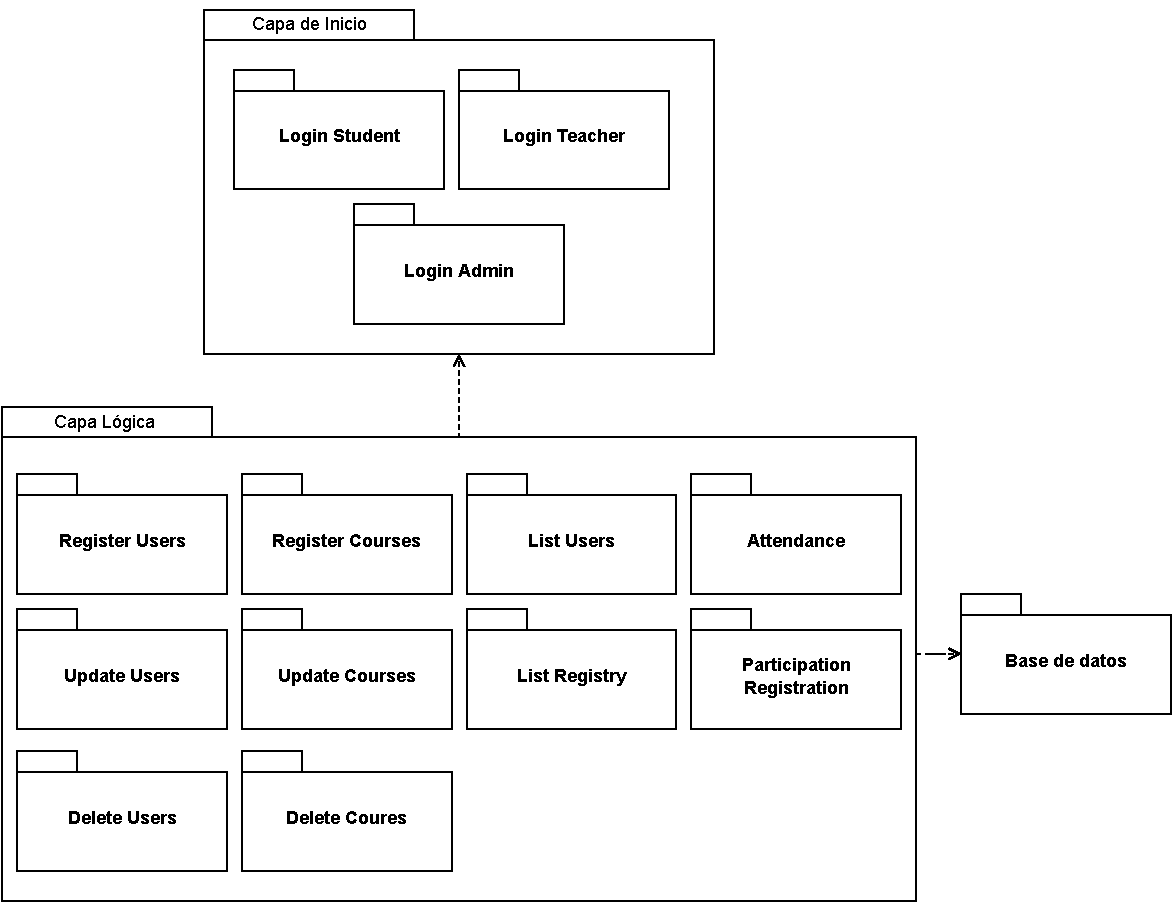
\includegraphics[width=1\textwidth]{assets/arq3.pdf}
    \caption{Arquitectura de la aplicación}
    \label{fig:arquitectura}
\end{figure}

\subsubsection{Base de datos}
\begin{figure}[H]
    \centering
    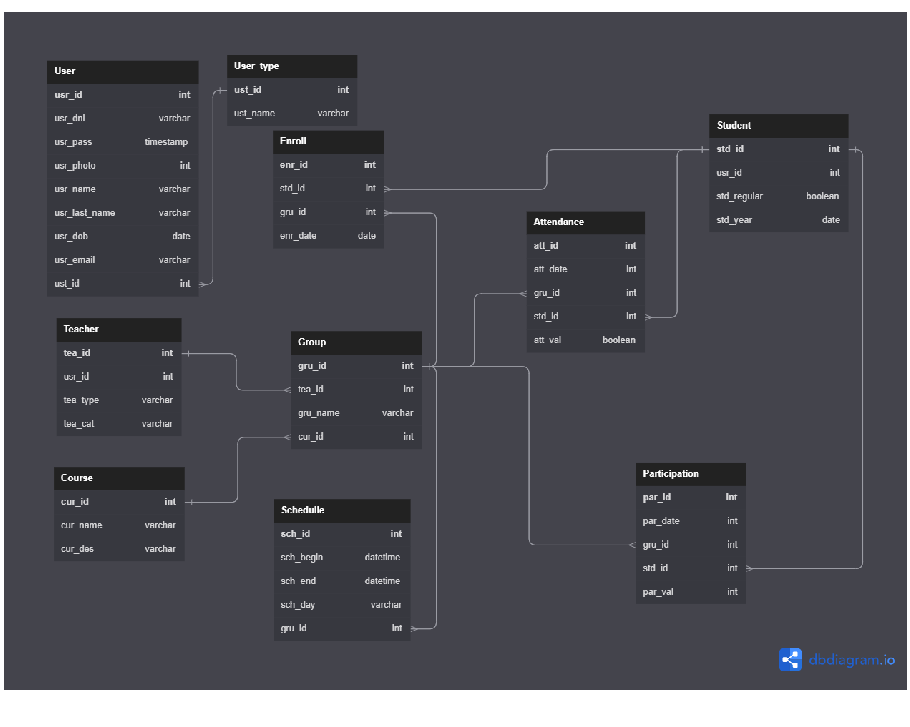
\includegraphics{assets/db.pdf}
    \caption{Diagrama de la base de datos}
    \label{fig:db}
\end{figure}
\subsection{Documentación de endpoints}

% Attendance endpoints

\subsubsection{Attendance}
\begin{enumerate}[i.]
    \item \textbf{Crear Attendance}
    \begin{itemize}
        \item http://127.0.0.1:8002/Attendance/create\_attendance.
        \item Donde va a crear una nueva Attendance en la base de datos.
        \item Request y Response:
        \item 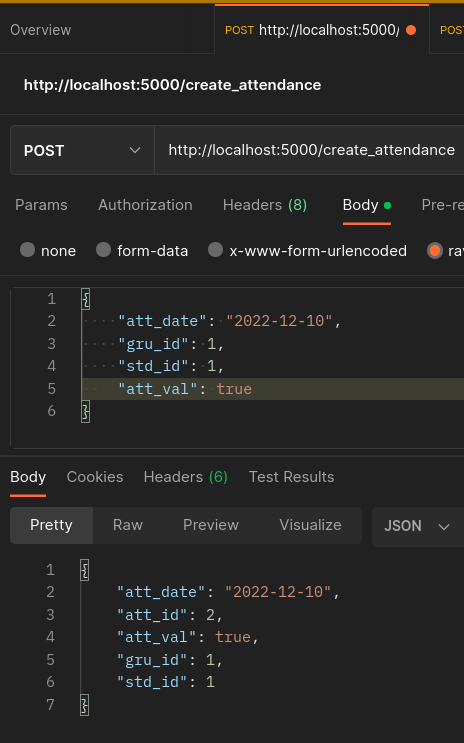
\includegraphics[scale=.5]{assets/attendance/create.png}
        \item Fields:
        \begin{table}[H] \centering \begin{tabular}{|c|c|c|l|} \hline \textbf{Field}
        & \textbf{Type} & \textbf{Required?} &
        \multicolumn{1}{c|}{\textbf{Description}} \\ \hline \textit{att\_date} &
        int & required & La fecha que tiene el Attendance \\ \hline
        \textit{gru\_id} & int & required & El id del grupo que pertenece el
        Attendance \\ \hline \textit{std\_id} & int & required & El id del
        estudiante que pertenece el Attendance \\ \hline \textit{att\_val} &
        boolean & required & El valor que se le pone si asistió el estudiante \\
        \hline \end{tabular} \end{table}
        \item Post objects:
        \begin{table}[H] \centering \begin{tabular}{|c|c|l|} \hline \textbf{Field} &
        \textbf{Type} & \multicolumn{1}{c|}{\textbf{Description}} \\ \hline
        \textit{att\_id} & int & El identificador del Attendance \\ \hline
        \textit{att\_date} & int & La fecha que se creó el attendance \\ \hline
        \textit{gru\_id} & int & Un identificador para cada grupo registrado \\
        \hline \textit{std\_id} & int & Un identificador para cada estudiante
        registrado \\ \hline \multicolumn{1}{|l|}{\textit{att\_val}} &
        \multicolumn{1}{l|}{boolean} & El valor que se le pone si asistió el
        estudiante \\ \hline \end{tabular} \end{table}
        \item Errores posibles:
        \begin{table}[H] \centering \begin{tabular}{|c|c|l|} \hline \textbf{Error} &
        \textbf{Description} \\ \hline \textit{400 Bad Request} & Algún
        identificador especificado no existe \\ \hline
        \end{tabular}
        \end{table}
    \end{itemize}

    \item \textbf{Listar Attendance por ID}
    \begin{itemize}
        \item http://127.0.0.1:8002/Attendancde/attendance/id
        \item Donde ``id'' es el identificador del Attendance que se
        quiere especificar.
        \item Request y Response:
        \item 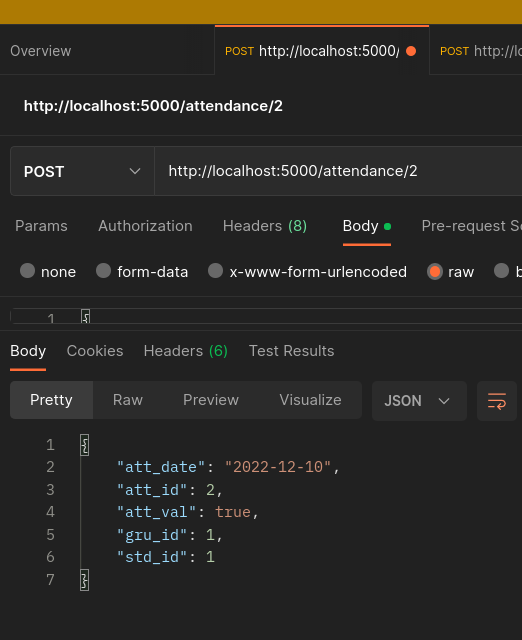
\includegraphics[scale=.5]{assets/attendance/atendance2.png}
        \item Post Objects:
        \begin{table}[H] \centering \begin{tabular}{|l|l|l|} \hline
        \multicolumn{1}{|c|}{\textbf{Field}} &
        \multicolumn{1}{c|}{\textbf{Type}} &
        \multicolumn{1}{c|}{\textbf{Description}} \\ \hline \textit{att\_id} &
        int & El identificador del Attendance \\ \hline \textit{att\_date} & int
        & La fecha que se creó el attendance \\ \hline \textit{gru\_id} & int &
        Un identificador para cada grupo registrado \\ \hline \textit{std\_id} &
        int & Un identificador para cada estudiante registrado \\ \hline
        \textit{att\_val} & boolean & El valor que se le pone si asistió el
        estudiante \\ \hline \end{tabular} \end{table}
        \item Errores posibles:
        \begin{table}[H] \centering \begin{tabular}{|c|c|l|} \hline \textbf{Error} &
        \textbf{Description} \\ \hline \textit{400 Bad Request} & El
        identificador especificado no existe. \\ \hline
        \end{tabular} \end {table}
    \end{itemize}

    \item \textbf{Listar Attendance}
    \begin{itemize}
        \item http://127.0.0.1:8002/Attendancde/attendances
        \item Donde se va a listar todas las Attendance en la base de datos.
        \item Request y Response:
        \item 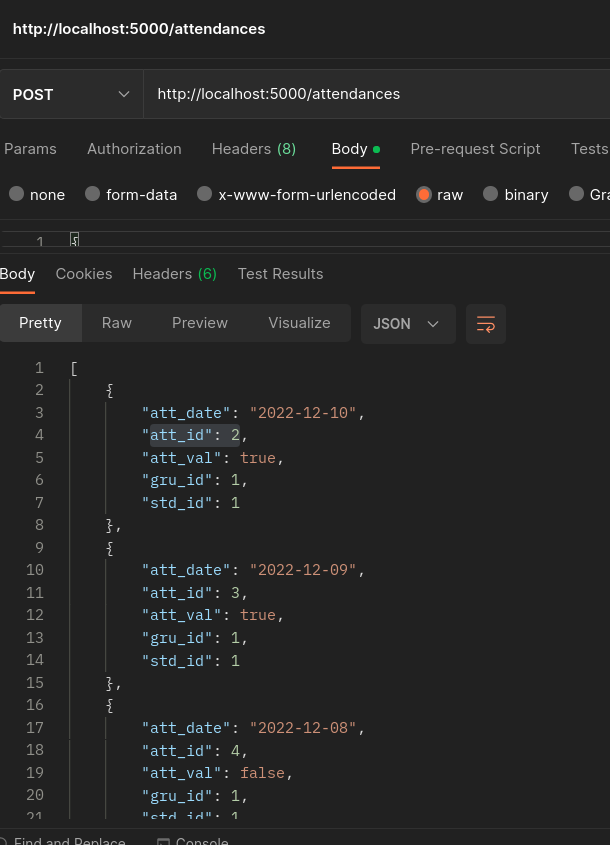
\includegraphics[scale=.5]{assets/attendance/atendances.png}
        \item Post objects:
        \begin{table}[H] \centering \begin{tabular}{|l|l|l|} \hline
        \multicolumn{1}{|c|}{\textbf{Field}} &
        \multicolumn{1}{c|}{\textbf{Type}} &
        \multicolumn{1}{c|}{\textbf{Description}} \\ \hline \textit{att\_id} &
        int & El identificador del Attendance \\ \hline \textit{att\_date} & int
        & La fecha que se creó el attendance \\ \hline \textit{gru\_id} & int &
        Un identificador para cada grupo registrado \\ \hline \textit{std\_id} &
        int & Un identificador para cada estudiante registrado \\ \hline
        \textit{att\_val} & boolean & El valor que se le pone si asistió el
        estudiante \\ \hline \end{tabular} \end{table}
    \end{itemize}

    \item \textbf{Actualizar Attendance}
    \begin{itemize}
        \item http://127.0.0.1:8002/Attendancde/update\_attendance/id
        \item Donde se va a actualizar el Attendance del ID especificado.
        \item Request y Response:
        \item 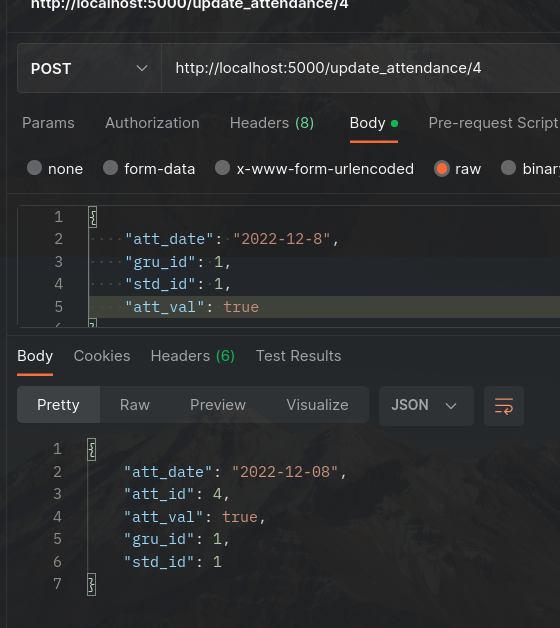
\includegraphics[scale=.5]{assets/attendance/update.png}
        \item Fields
        \begin{table}[H] \centering \begin{tabular}{|l|l|l|l|} \hline
        \multicolumn{1}{|c|}{\textbf{Field}} &
        \multicolumn{1}{c|}{\textbf{Type}} &
        \multicolumn{1}{c|}{\textbf{Required?}} &
        \multicolumn{1}{c|}{\textbf{Description}} \\ \hline \textit{att\_date} &
        int & required & La fecha que tiene el Attendance \\ \hline
        \textit{gru\_id} & int & required & El id del grupo que pertenece el
        Attendance \\ \hline \textit{std\_id} & int & required & El id del
        estudiante que pertenece el Attendance \\ \hline \textit{att\_val} &
        boolean & required & El valor que se le pone si asistió el estudiante \\
        \hline \end{tabular} \end{table}
        \item Post objects:
        \begin{table}[H] \centering \begin{tabular}{|l|l|l|} \hline
        \multicolumn{1}{|c|}{\textbf{Field}} &
        \multicolumn{1}{c|}{\textbf{Type}} &
        \multicolumn{1}{c|}{\textbf{Description}} \\ \hline \textit{att\_id} &
        int & El identificador del Attendance \\ \hline \textit{att\_date} & int
        & La fecha que se creó el attendance \\ \hline \textit{gru\_id} & int &
        Un identificador para cada grupo registrado \\ \hline \textit{std\_id} &
        int & Un identificador para cada estudiante registrado \\ \hline
        \textit{att\_val} & boolean & El valor que se le pone si asistió el
        estudiante \\ \hline \end{tabular} \end{table}
        \item Errores posibles:
        \begin{table}[H] \centering \begin{tabular}{|c|c|l|} \hline \textbf{Error} &
        \textbf{Description} \\ \hline \textit{400 Bad Request} & Algun identificador
        especificado no existe. \\ \hline \end{tabular} \end{table}
        
    \end{itemize}

    \item \textbf{Eliminar Attendance}
    \begin{itemize}
        \item http://127.0.0.1:8002/Attendancde/delete\_attendance/id
        \item Donde se va a eliminar el Attendance del ID especificado.
        \item Request y Response:
        \item 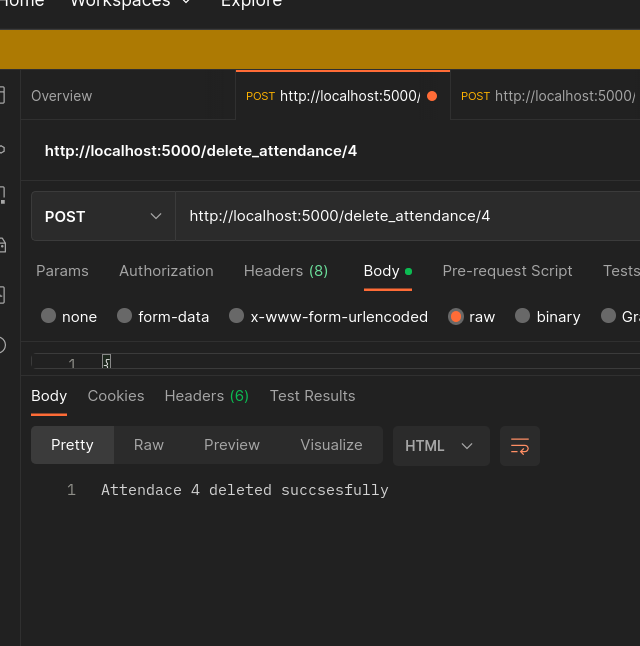
\includegraphics[scale=.5]{assets/attendance/delete.png}
        \item Errores posibles:
        \begin{table}[H] \centering \begin{tabular}{|c|c|l|} \hline \textbf{Error}
        & \textbf{Description} \\ \hline \textit{400 Bad Request} & Algun
        identificador especificado no existe. \\ \hline \end{tabular}
        \end{table}
    \end{itemize}
\end{enumerate}

% Course endpoints
\subsubsection{Course}
\begin{enumerate}
    \item \textbf{Crear Course}
    \begin{itemize}
        \item http://127.0.0.1:8002/Course/create\_course
        \item Donde va a crear un nuevo Curso en la base de datos.
        \item Request y Response:
        \item 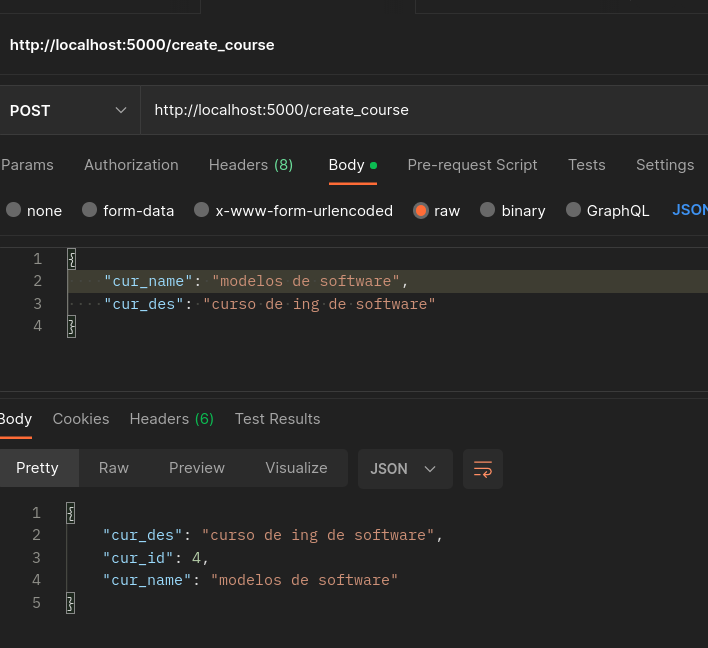
\includegraphics[scale=.5]{assets/course/create.png}
        \begin{table}[H] \centering \begin{tabular}{|l|l|l|l|} \hline
        \multicolumn{1}{|c|}{\textbf{Field}} &
        \multicolumn{1}{c|}{\textbf{Type}} &
        \multicolumn{1}{c|}{\textbf{Required?}} &
        \multicolumn{1}{c|}{\textbf{Description}} \\ \hline \textit{cur\_name} &
        varchar & required & El nombre que tiene el curso \\ \hline
        \textit{cur\_des} & varchar & required & La descripción general que va a
        tener el curso. \\ \hline \end{tabular} \end{table}
        \item Post objects:
        \begin{table}[H] \centering \begin{tabular}{|l|l|l|} \hline
        \multicolumn{1}{|c|}{\textbf{Field}} &
        \multicolumn{1}{c|}{\textbf{Type}} &
        \multicolumn{1}{c|}{\textbf{Description}} \\ \hline \textit{cur\_id} &
        int & El identificador que tiene el curso \\ \hline \textit{cur\_name} &
        varchar & Una cadena de texto que representa el nombre del curso \\
        \hline \textit{cur\_des} & varchar & Una cadena de texto que representa
        la descripción del curso \\ \hline \end{tabular} \end{table}
    \end{itemize}

    \item \textbf{Listar Course por ID}
    \begin{itemize}
        \item http://127.0.0.1:8002/Course/attendance/id
        \item Donde ``id'' es el identificador del Course que se quiere
        especificar.
        \item Request y Response:
        \item 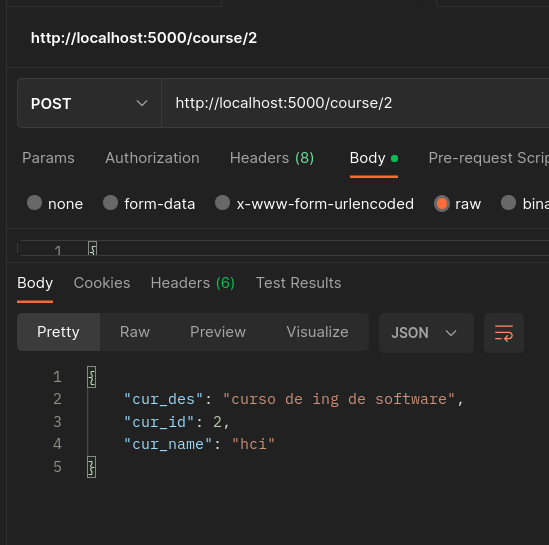
\includegraphics[scale=.5]{assets/course/course2.png}
        \item Post Objects:
        \begin{table}[H] \centering \begin{tabular}{|l|l|l|} \hline
        \multicolumn{1}{|c|}{\textbf{Field}} &
        \multicolumn{1}{c|}{\textbf{Type}} &
        \multicolumn{1}{c|}{\textbf{Description}} \\ \hline \textit{cur\_id} &
        int & El identificador que tiene el curso \\ \hline \textit{cur\_name} &
        varchar & Una cadena de texto que representa el nombre del curso \\
        \hline \textit{cur\_des} & varchar & Una cadena de texto que representa
        la descripción del curso \\ \hline \end{tabular} \end{table}
        \item Errores posibles:
        \begin{table}[H] \centering \begin{tabular}{|c|c|l|} \hline \textbf{Error Code} & \textbf{Description}
        \\ \hline \textit{400 Bad Request} & Algun identificador especificado
        no existe. \\ \hline \end{tabular} \end{table}
    \end{itemize}

    \item \textbf{Listar Courses}
    \begin{itemize}
        \item http://127.0.0.1:8002/Course/attendances
        \item Donde se va a listar a todos los Courses de la base de
        datos.
        \item Request y Response:
        \item 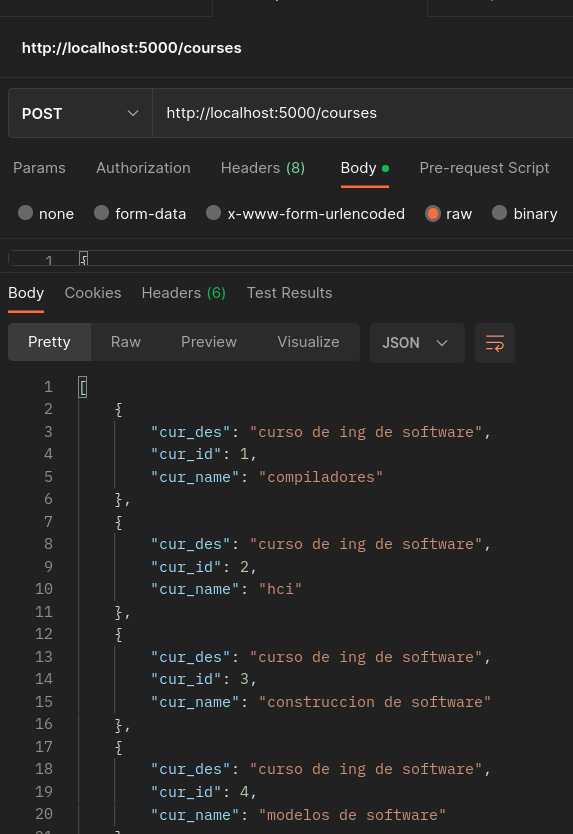
\includegraphics[scale=.5]{assets/course/courses.png}
        \item Post Obejcts: 
        \begin{table}[H] \centering \begin{tabular}{|l|l|l|} \hline
        \multicolumn{1}{|c|}{\textbf{Field}} &
        \multicolumn{1}{c|}{\textbf{Type}} &
        \multicolumn{1}{c|}{\textbf{Description}} \\ \hline \textit{cur\_id} &
        int & El identificador que tiene el curso \\ \hline \textit{cur\_name} &
        varchar & Una cadena de texto que representa el nombre del curso \\
        \hline \textit{cur\_des} & varchar & Una cadena de texto que representa
        la descripción del curso \\ \hline \end{tabular} \end{table}
    \end{itemize}

    \item \textbf{Actualizar Course}
    \begin{itemize}
        \item http://127.0.0.1:8002/Course/update\_course/id
        \item Donde se va a actualizar el Course del ID especificado.
        \item Request y Response:
        \item 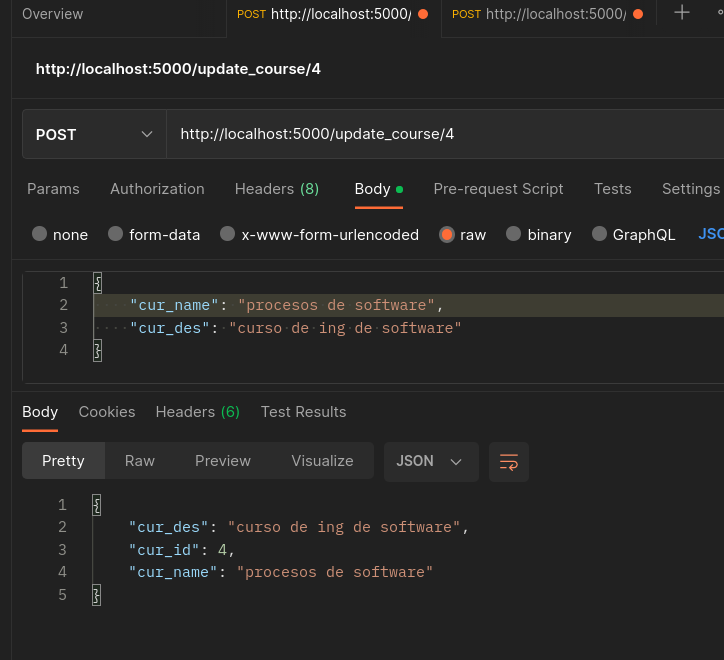
\includegraphics[scale=.5]{assets/course/update.png}
        \item Fields
        \begin{table}[H] \centering \begin{tabular}{|l|l|l|l|} \hline
        \multicolumn{1}{|c|}{\textbf{Field}} &
        \multicolumn{1}{c|}{\textbf{Type}} &
        \multicolumn{1}{c|}{\textbf{Required?}} &
        \multicolumn{1}{c|}{\textbf{Description}} \\ \hline \textit{cur\_name} &
        varchar & required & El nombre que tiene el curso \\ \hline
        \textit{cur\_des} & varchar & required & La descripción general que va a
        tener el curso. \\ \hline \end{tabular} \end{table}

        \item Post objects:
        \begin{table}[H] \centering \begin{tabular}{|l|l|l|} \hline
        \multicolumn{1}{|c|}{\textbf{Field}} &
        \multicolumn{1}{c|}{\textbf{Type}} &
        \multicolumn{1}{c|}{\textbf{Description}} \\ \hline \textit{cur\_id} &
        int & El identificador que tiene el curso \\ \hline \textit{cur\_name} &
        varchar & Una cadena de texto que representa el nombre del curso \\
        \hline \textit{cur\_des} & varchar & Una cadena de texto que representa
        la descripción del curso \\ \hline \end{tabular} \end{table}
    \end{itemize}

    \item \textbf{Eliminar Course}
    \begin{itemize}
        \item http://127.0.0.1:8002/Course/delete\_course/id
        \item Donde se va a eliminar el Course del ID especificado.
        \item Request y Response:
        \item 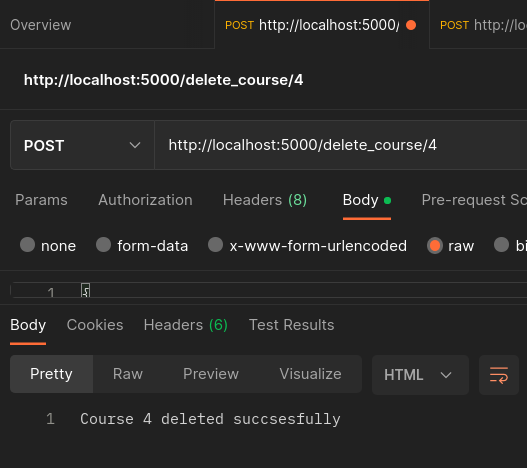
\includegraphics[scale=.5]{assets/course/delete.png}
        \item Errores posibles
        \item Errores posibles: \begin{table}[H] \centering
        \begin{tabular}{|c|c|l|} \hline \textbf{Error Code} &
        \textbf{Description} \\ \hline \textit{400 Bad Request} & Algun
        identificador especificado no existe. \\ \hline \end{tabular}
        \end{table}
    \end{itemize}

\end{enumerate}


%  Enroll endpoints
\subsubsection{Enroll}
\begin{enumerate}
    \item \textbf{Crear Enroll}
    \begin{itemize}
        \item http://127.0.0.1:8002/Enroll/create\_enroll
        \item Donde va a crear un nuevo Enroll en la base de datos.
        \item Request y Response:
        \item 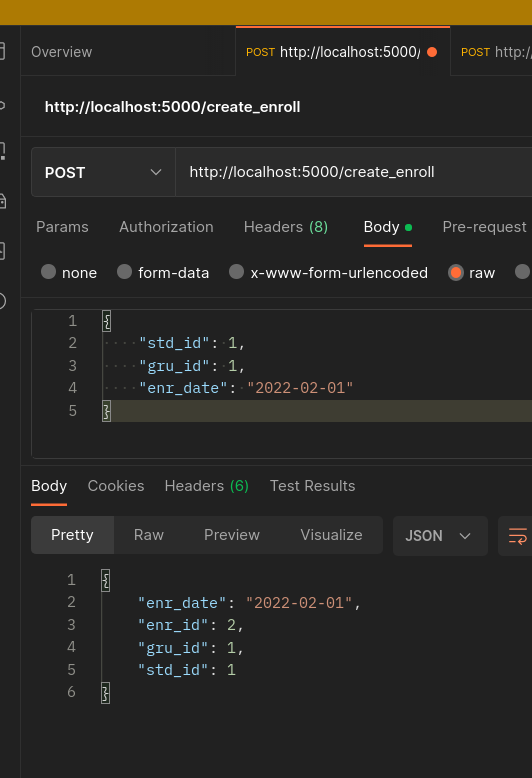
\includegraphics[scale=.5]{assets/enroll/create.png}
        \item Fields:
        \begin{table}[H] \centering \begin{tabular}{|l|l|l|l|} \hline
        \multicolumn{1}{|c|}{\textbf{Field}} &
        \multicolumn{1}{c|}{\textbf{Type}} &
        \multicolumn{1}{c|}{\textbf{Required?}} &
        \multicolumn{1}{c|}{\textbf{Description}} \\ \hline \textit{std\_id} &
        int & required & El id del estudiante al que pertenece el enroll \\
        \hline \textit{gru\_id} & int & required & El id del grupo al que
        pertenece el Enroll \\ \hline enr\_date & date & required & La fecha que
        tiene el Enroll \\ \hline \end{tabular} \end{table}
        \item Post objects:
        \begin{table}[H] \centering \begin{tabular}{|l|l|l|} \hline
        \multicolumn{1}{|c|}{\textbf{Field}} &
        \multicolumn{1}{c|}{\textbf{Type}} &
        \multicolumn{1}{c|}{\textbf{Description}} \\ \hline \textit{enr\_id} &
        int & El identificador que tiene el enroll \\ \hline \textit{std\_id} &
        int & Un identificador para cada estudiante registrado \\ \hline
        \textit{gru\_id} & int & Un identificador para cada grupo registrado \\
        \hline enr\_date & date & La fecha que se creó el enroll \\ \hline
        \end{tabular} \end{table}
        \item Errores posibles:
        \begin{table}[H] \centering \begin{tabular}{|c|c|l|} \hline \textbf{Error Code}
        & \textbf{Description} \\ \hline \textit{400 Bad Request} & Algun 
        identificador especificado no existe. \\ \hline \end{tabular}
        \end{table}
    \end{itemize}

    \item \textbf{Listar Enroll por ID}
    \begin{itemize}
        \item http://127.0.0.1:8002/Enroll/enroll/id
        \item Donde ``id'' es el identificador del Enroll que se quiere
        especificar.
        \item Request y Response:
        \item 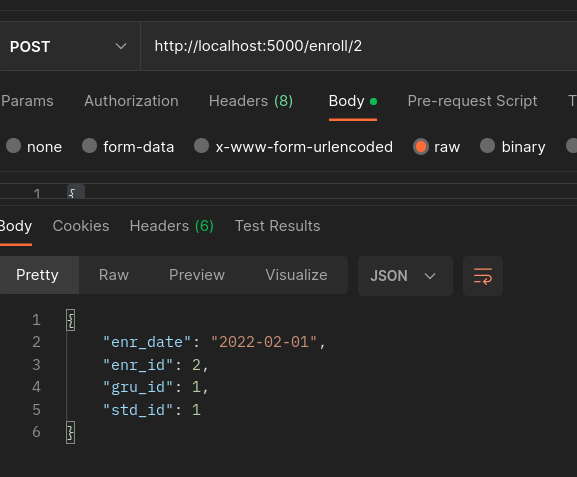
\includegraphics[scale=.5]{assets/enroll/enroll2.png}
        \item Post objects:
        \begin{table}[H] \centering \begin{tabular}{|l|l|l|} \hline
        \multicolumn{1}{|c|}{\textbf{Field}} &
        \multicolumn{1}{c|}{\textbf{Type}} &
        \multicolumn{1}{c|}{\textbf{Description}} \\ \hline \textit{enr\_id} &
        int & El identificador que tiene el enroll \\ \hline \textit{std\_id} &
        int & Un identificador para cada estudiante registrado \\ \hline
        \textit{gru\_id} & int & Un identificador para cada grupo registrado \\
        \hline enr\_date & date & La fecha que se creó el enroll \\ \hline
        \end{tabular} \end{table}
        \item Errores posibles: \begin{table}[H] \centering
        \begin{tabular}{|c|c|l|} \hline \textbf{Error Code} &
        \textbf{Description} \\ \hline \textit{400 Bad Request} & Algun
        identificador especificado no existe. \\ \hline \end{tabular} \end{table}
    \end{itemize}

    \item \textbf{Actualizar Enroll}
    \begin{itemize}
        \item http://127.0.0.1:8002/Enroll/update\_enroll/id
        \item Donde se va a actualizar el Enroll del ID especificado.
        \item Request y Response:
        \item 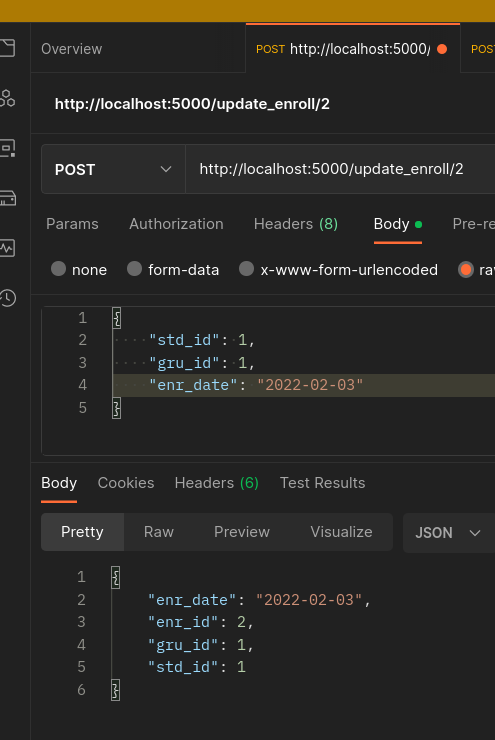
\includegraphics[scale=.5]{assets/enroll/update.png}
        \item Fields:
        \begin{table}[H] \centering \begin{tabular}{|l|l|l|l|} \hline
        \multicolumn{1}{|c|}{\textbf{Field}} &
        \multicolumn{1}{c|}{\textbf{Type}} &
        \multicolumn{1}{c|}{\textbf{Required?}} &
        \multicolumn{1}{c|}{\textbf{Description}} \\ \hline \textit{std\_id} &
        int & required & El id del estudiante al que pertenece el enroll \\
        \hline \textit{gru\_id} & int & required & El id del grupo al que
        pertenece el Enroll \\ \hline enr\_date & date & required & La fecha que
        tiene el Enroll \\ \hline \end{tabular} \end{table}
        \item Post objects:
        \begin{table}[H] \centering \begin{tabular}{|l|l|l|} \hline
        \multicolumn{1}{|c|}{\textbf{Field}} &
        \multicolumn{1}{c|}{\textbf{Type}} &
        \multicolumn{1}{c|}{\textbf{Description}} \\ \hline \textit{enr\_id} &
        int & El identificador que tiene el enroll \\ \hline \textit{std\_id} &
        int & Un identificador para cada estudiante registrado \\ \hline
        \textit{gru\_id} & int & Un identificador para cada grupo registrado \\
        \hline enr\_date & date & La fecha que se creó el enroll \\ \hline
        \end{tabular} \end{table}
        \item Errores posibles: \begin{table}[H] \centering
        \begin{tabular}{|c|c|l|} \hline \textbf{Error Code} &
        \textbf{Description} \\ \hline \textit{400 Bad Request} & Algun
        identificador especificado no existe. \\ \hline \end{tabular}
        \end{table}
        
    \end{itemize}

    \item \textbf{Eliminar Enroll}
    \begin{itemize}
        \item http://127.0.0.1:8002/Enroll/delete\_enroll/id
        \item Donde se va a eliminar el Enroll del ID especificado.
        \item Request y Response:
        \item 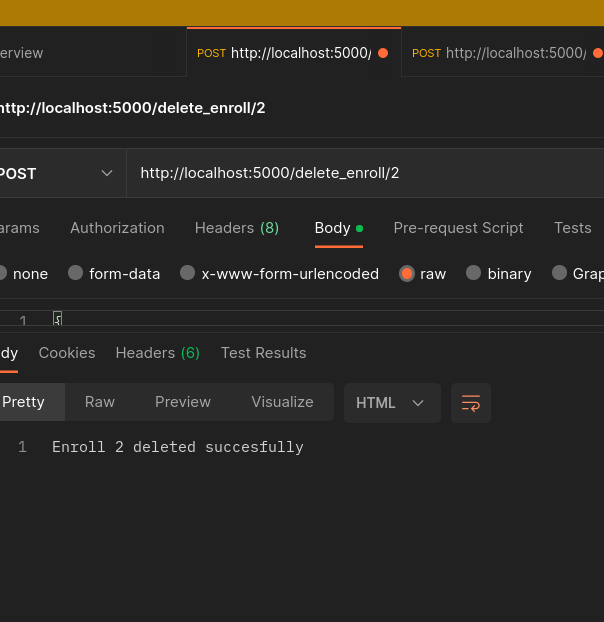
\includegraphics[scale=.5]{assets/enroll/delete.png}
        \item Errores posibles: \begin{table}[H] \centering
        \begin{tabular}{|c|c|l|} \hline \textbf{Error Code} &
        \textbf{Description} \\ \hline \textit{400 Bad Request} & Algun
        identificador especificado no existe. \\ \hline \end{tabular}
        \end{table}
    \end{itemize}
\end{enumerate}

% group endpoints
\subsection{Group}
\begin{enumerate}
    \item \textbf{Crear Group}
    \begin{itemize}
        \item http://127.0.0.1:8002/Group/create\_group
        \item Donde va a crear un nuevo Group en la base de datos.
        \item Request y Response:
        \item 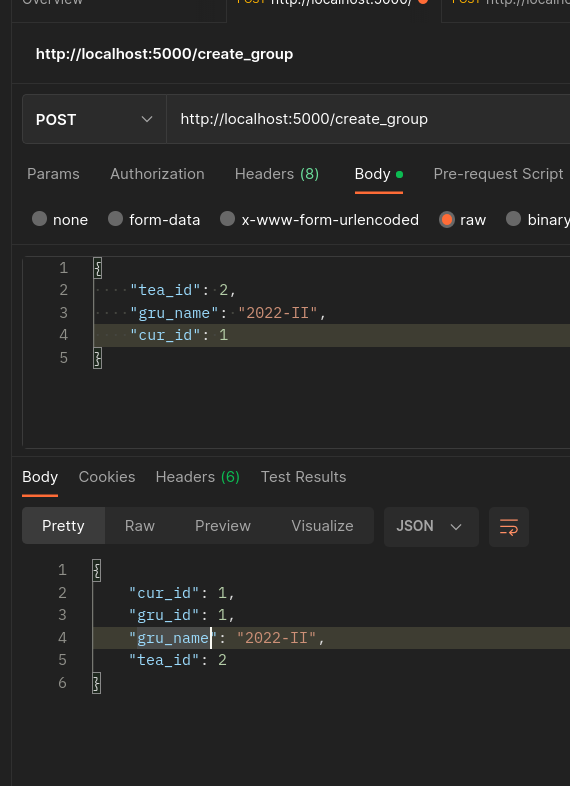
\includegraphics[scale=.5]{assets/group/create.png}
        \item Fields
        \begin{table}[H] \centering \begin{tabular}{|l|l|l|l|} \hline
        \multicolumn{1}{|c|}{\textbf{Field}} &
        \multicolumn{1}{c|}{\textbf{Type}} &
        \multicolumn{1}{c|}{\textbf{Required?}} &
        \multicolumn{1}{c|}{\textbf{Description}} \\ \hline
        \textit{\textbf{tea\_id}} & int & required & El id del teacher al que
        contiene el Group \\ \hline \textit{gru\_name} & varchar & required & El
        nombre que tiene el grupo \\ \hline cur\_id & date & required & El id
        del curso al que contiene el Group \\ \hline \end{tabular} \end{table}
        \item Post objects:
        \begin{table}[H] \centering \begin{tabular}{|l|l|l|} \hline
        \multicolumn{1}{|c|}{\textbf{Field}} &
        \multicolumn{1}{c|}{\textbf{Type}} &
        \multicolumn{1}{c|}{\textbf{Description}} \\ \hline \textit{gru\_id} &
        int & El identificador que tiene el grupo \\ \hline \textit{tea\_id} &
        int & Un identificador para cada teacher registrado \\ \hline
        \textit{gru\_name} & varchar & Una cadena de texto que representa el
        nombre del grupo \\ \hline cur\_id & date & Un identificador para cada
        curso registrado \\ \hline \end{tabular} \end{table}
        \item Errores posibles: \begin{table}[H] \centering
        \begin{tabular}{|c|c|l|} \hline \textbf{Error Code} &
        \textbf{Description} \\ \hline \textit{400 Bad Request} & Algun
        identificador especificado no existe. \\ \hline \end{tabular}
        \end{table}
    \end{itemize}

    \item \textbf{Listar Group por ID}
    \begin{itemize}
        \item http://127.0.0.1:8002/Group/group/id
        \item Donde ``id'' es el identificador del Group que se quiere
        especificar.
        \item Request y Response:
        \item 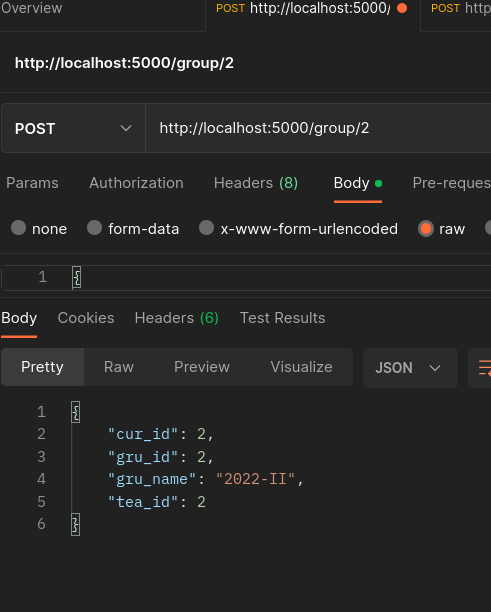
\includegraphics[scale=.5]{assets/group/group2.png}
        \item Post objects:
        \begin{table}[H] \centering \begin{tabular}{|l|l|l|} \hline
        \multicolumn{1}{|c|}{\textbf{Field}} &
        \multicolumn{1}{c|}{\textbf{Type}} &
        \multicolumn{1}{c|}{\textbf{Description}} \\ \hline \textit{gru\_id} &
        int & El identificador que tiene el grupo \\ \hline \textit{tea\_id} &
        int & Un identificador para cada teacher registrado \\ \hline
        \textit{gru\_name} & varchar & Una cadena de texto que representa el
        nombre del grupo \\ \hline cur\_id & date & Un identificador para cada
        curso registrado \\ \hline \end{tabular} \end{table}
        \item Errores posibles:
        \begin{table}[H] \centering \begin{tabular}{|c|c|l|} \hline \textbf{Error
        Code} & \textbf{Description} \\ \hline \textit{400 Bad Request} & Algun
        identificador especificado no existe. \\ \hline \end{tabular}
        \end{table}
    \end{itemize}

    \item \textbf{Listar Group}
    \begin{itemize}
        \item http://127.0.0.1:8002/Group/groups
        \item Donde se va a listar a todos los Groups de la base de
        datos.
        \item Request y Response:
        \item 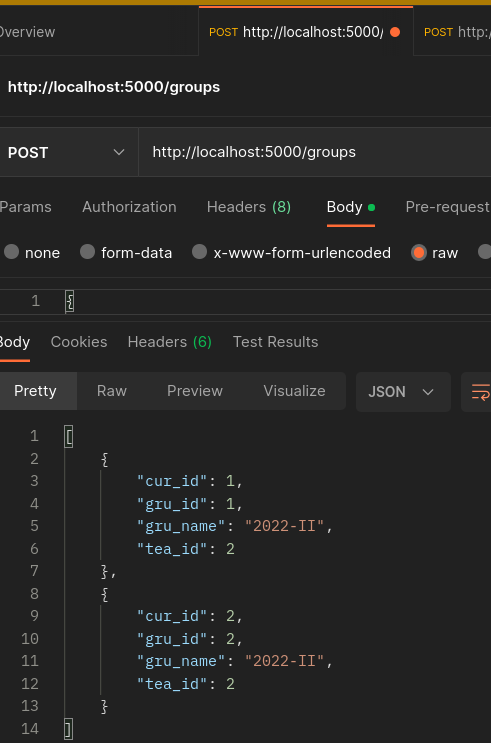
\includegraphics[scale=.5]{assets/group/groups.png}
        \item Post objects:
        \begin{table}[H] \centering \begin{tabular}{|l|l|l|} \hline
        \multicolumn{1}{|c|}{\textbf{Field}} &
        \multicolumn{1}{c|}{\textbf{Type}} &
        \multicolumn{1}{c|}{\textbf{Description}} \\ \hline \textit{gru\_id} &
        int & El identificador que tiene el grupo \\ \hline \textit{tea\_id} &
        int & Un identificador para cada teacher registrado \\ \hline
        \textit{gru\_name} & varchar & Una cadena de texto que representa el
        nombre del grupo \\ \hline cur\_id & date & Un identificador para cada
        curso registrado \\ \hline \end{tabular} \end{table}
    \end{itemize}

    \item \textbf{Actualizar Group}
    \begin{itemize}
        \item http://127.0.0.1:8002/Group/update\_group
        \item Donde se va a actualizar el Group del ID especificado.
        \item Request y Response
        \item 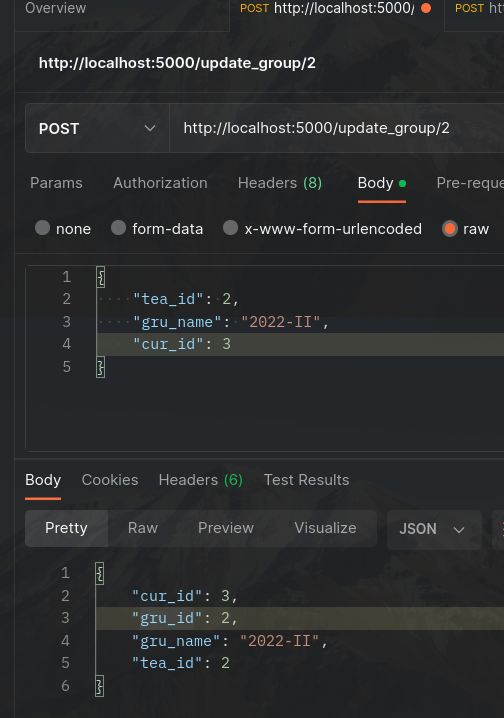
\includegraphics[scale=.5]{assets/group/update.png}
        \item Fields
        \begin{table}[H] \centering \begin{tabular}{|l|l|l|l|} \hline
        \multicolumn{1}{|c|}{\textbf{Field}} &
        \multicolumn{1}{c|}{\textbf{Type}} &
        \multicolumn{1}{c|}{\textbf{Required?}} &
        \multicolumn{1}{c|}{\textbf{Description}} \\ \hline
        \textit{\textbf{tea\_id}} & int & required & El id del teacher al que
        contiene el Group \\ \hline \textit{gru\_name} & varchar & required & El
        nombre que tiene el grupo \\ \hline cur\_id & date & required & El id
        del curso al que contiene el Group \\ \hline \end{tabular} \end{table}
        \item Post objects:
        \begin{table}[H] \centering \begin{tabular}{|l|l|l|} \hline
        \multicolumn{1}{|c|}{\textbf{Field}} &
        \multicolumn{1}{c|}{\textbf{Type}} &
        \multicolumn{1}{c|}{\textbf{Description}} \\ \hline \textit{gru\_id} &
        int & El identificador que tiene el grupo \\ \hline \textit{tea\_id} &
        int & Un identificador para cada teacher registrado \\ \hline
        \textit{gru\_name} & varchar & Una cadena de texto que representa el
        nombre del grupo \\ \hline cur\_id & date & Un identificador para cada
        curso registrado \\ \hline \end{tabular} \end{table}
        \item Errores posibles: \begin{table}[H] \centering
        \begin{tabular}{|c|c|l|} \hline \textbf{Error Code} &
        \textbf{Description} \\ \hline \textit{400 Bad Request} & Algun
        identificador especificado no existe. \\ \hline \end{tabular}
        \end{table}
    \end{itemize}

    \item \textbf{Eliminar Group}
    \begin{itemize}
        \item http://127.0.0.1:8002/Group/delete\_group
        \item Donde se va a eliminar el Group del ID especificado.
        \item Request y Response:
        \item 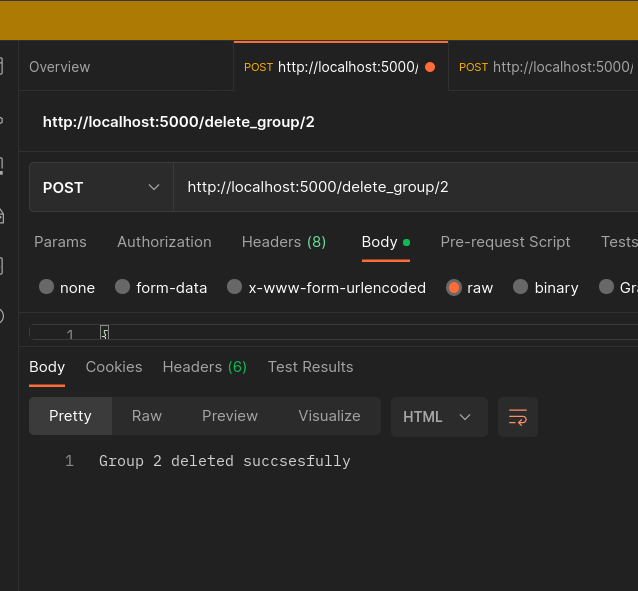
\includegraphics[scale=.5]{assets/group/delete.png}
        \item Errores posibles:
        \begin{table}[H] \centering \begin{tabular}{|c|c|l|} \hline \textbf{Error
        Code} & \textbf{Description} \\ \hline \textit{400 Bad Request} & Algun
        identificador especificado no existe. \\ \hline \end{tabular}
        \end{table}
    \end{itemize}
\end{enumerate}

\subsection{Participation}
\begin{enumerate}
    \item \textbf{Crear Participation}
    \begin{itemize}
        \item http://127.0.0.1:8002/Participation/create\_participation
        \item Donde va a crear una nueva Participation en la base de datos.
        \item Request y Response:
        \item 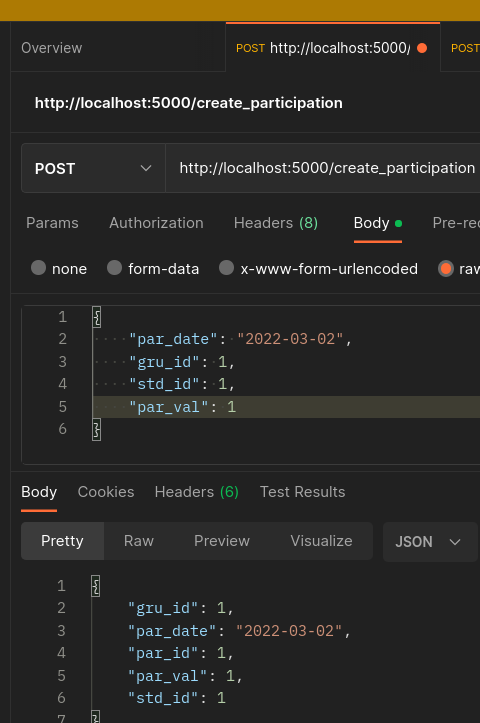
\includegraphics[scale=.5]{assets/participation/create.png}
        \item Fields
        \begin{table}[H] \centering \begin{tabular}{|l|l|l|l|} \hline
        \multicolumn{1}{|c|}{\textbf{Field}} &
        \multicolumn{1}{c|}{\textbf{Type}} &
        \multicolumn{1}{c|}{\textbf{Required?}} &
        \multicolumn{1}{c|}{\textbf{Description}} \\ \hline par\_date & int &
        required & La fecha que tiene la Participation \\ \hline gru\_id & int &
        required & El id del grupo que pertenece la Participation \\ \hline
        std\_id & int & required & El id del estudiante que pertenece la
        Participation \\ \hline par\_val & int & required & El valor que tiene
        el total de Participations \\ \hline \end{tabular} \end{table}
        \item Post objects:
        \begin{table}[H] \centering \begin{tabular}{|l|l|l|} \hline
        \multicolumn{1}{|c|}{\textbf{Field}} &
        \multicolumn{1}{c|}{\textbf{Type}} &
        \multicolumn{1}{c|}{\textbf{Description}} \\ \hline par\_id & int & El
        identificador de la Participation \\ \hline par\_date & int & La fecha
        que se creó la Participation \\ \hline gru\_id & int & Un identificador
        para cada grupo registrado \\ \hline std\_id & int & Un identificador
        para cada estudiante registrado \\ \hline par\_val & int & El valor que
        tiene el total de Participations \\ \hline \end{tabular} \end{table}
        \item Errores posibles: \begin{table}[H] \centering
        \begin{tabular}{|c|c|l|} \hline \textbf{Error Code} &
        \textbf{Description} \\ \hline \textit{400 Bad Request} & Algun
        identificador especificado no existe. \\ \hline \end{tabular}
        \end{table}
    \end{itemize}

    \item \textbf{Listar Participation por ID}
    \begin{itemize}
        \item http://127.0.0.1:8002/Participation/participation/id
        \item Donde ``id'' es el identificador de la Participation que
        se quiere especificar.
        \item Request y Response:
        \item 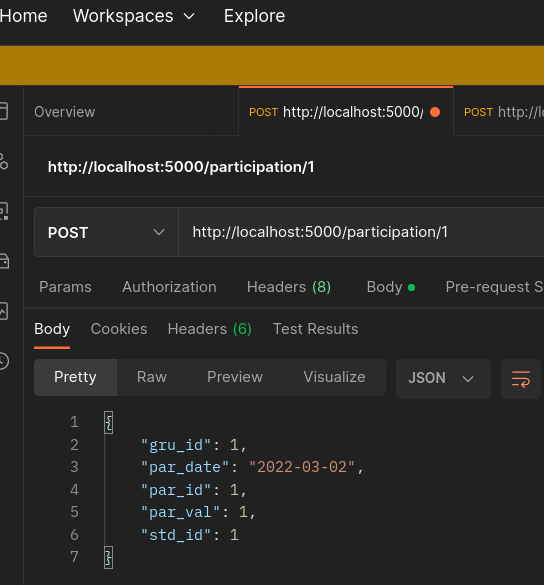
\includegraphics[scale=.5]{assets/participation/participations1.png}
        \item Post Obejcts
        \begin{table}[H] \centering \begin{tabular}{|l|l|l|} \hline
        \multicolumn{1}{|c|}{\textbf{Field}} &
        \multicolumn{1}{c|}{\textbf{Type}} &
        \multicolumn{1}{c|}{\textbf{Description}} \\ \hline par\_id & int & El
        identificador de la Participation \\ \hline par\_date & int & La fecha
        que se creó la Participation \\ \hline gru\_id & int & Un identificador
        para cada grupo registrado \\ \hline std\_id & int & Un identificador
        para cada estudiante registrado \\ \hline par\_val & int & El valor que
        tiene el total de Participations \\ \hline \end{tabular} \end{table}
        \item Errores posibles: \begin{table}[H] \centering \begin{tabular}{|c|c|l|} \hline
        \textbf{Error Code} & \textbf{Description} \\ \hline \textit{400 Bad
        Request} & Algun identificador especificado no existe. \\ \hline
        \end{tabular} \end{table}
    \end{itemize}

    \item \textbf{Listar Participation}
    \begin{itemize}
        \item http://127.0.0.1:8002/Participation/participations
        \item Donde se va a listar a todas las Participations de la base
        de datos.
        \item Request y Response:
        \item 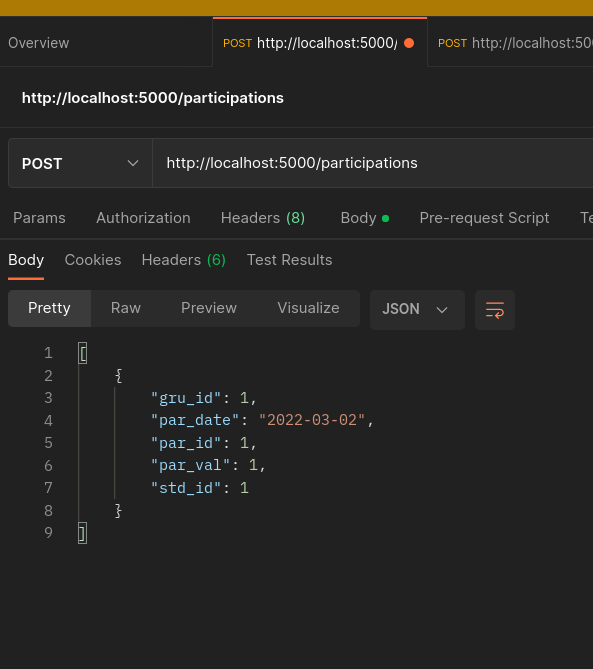
\includegraphics[scale=.5]{assets/participation/participations.png}
        \item Post objects
        \begin{table}[H] \centering \begin{tabular}{|l|l|l|} \hline
        \multicolumn{1}{|c|}{\textbf{Field}} &
        \multicolumn{1}{c|}{\textbf{Type}} &
        \multicolumn{1}{c|}{\textbf{Description}} \\ \hline par\_id & int & El
        identificador de la Participation \\ \hline par\_date & int & La fecha
        que se creó la Participation \\ \hline gru\_id & int & Un identificador
        para cada grupo registrado \\ \hline std\_id & int & Un identificador
        para cada estudiante registrado \\ \hline par\_val & int & El valor que
        tiene el total de Participations \\ \hline \end{tabular} \end{table}
    \end{itemize}

    \item \textbf{Actualizar Participation}
    \begin{itemize}
        \item http://127.0.0.1:8002/Participation/update\_participation/id
        \item Donde se va a eliminar la Participation del ID
        especificado
        \item Request y Response:
        \item 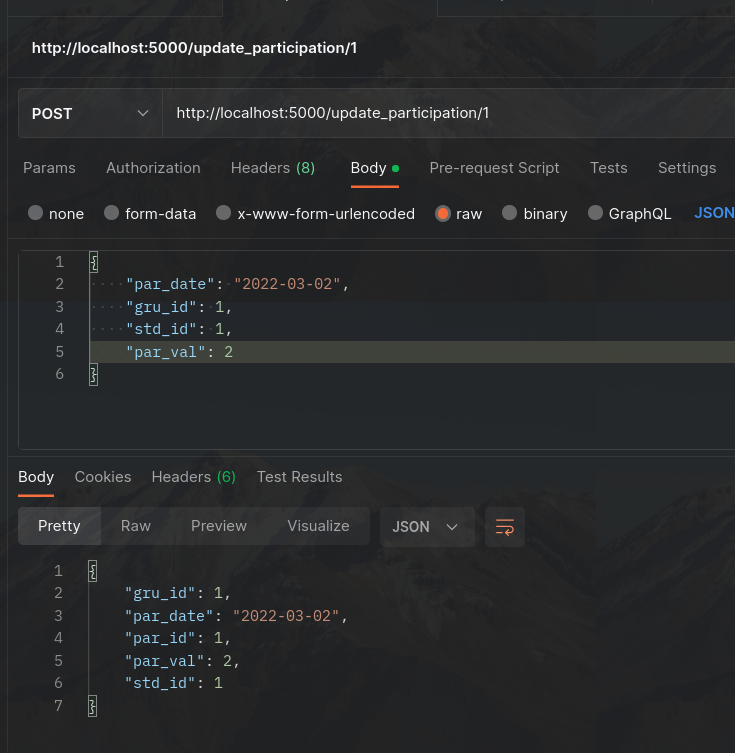
\includegraphics[scale=.5]{assets/participation/update.png}
        \item Fields:
        \begin{table}[H] \centering \begin{tabular}{|l|l|l|l|} \hline
        \multicolumn{1}{|c|}{\textbf{Field}} &
        \multicolumn{1}{c|}{\textbf{Type}} &
        \multicolumn{1}{c|}{\textbf{Required?}} &
        \multicolumn{1}{c|}{\textbf{Description}} \\ \hline par\_date & int &
        required & La fecha que tiene la Participation \\ \hline gru\_id & int &
        required & El id del grupo que pertenece la Participation \\ \hline
        std\_id & int & required & El id del estudiante que pertenece la
        Participation \\ \hline par\_val & int & required & El valor que tiene
        el total de Participations \\ \hline \end{tabular} \end{table} \item
        Post objects: \begin{table}[H] \centering \begin{tabular}{|l|l|l|} \hline
        \multicolumn{1}{|c|}{\textbf{Field}} &
        \multicolumn{1}{c|}{\textbf{Type}} &
        \multicolumn{1}{c|}{\textbf{Description}} \\ \hline par\_id & int & El
        identificador de la Participation \\ \hline par\_date & int & La fecha
        que se creó la Participation \\ \hline gru\_id & int & Un identificador
        para cada grupo registrado \\ \hline std\_id & int & Un identificador
        para cada estudiante registrado \\ \hline par\_val & int & El valor que
        tiene el total de Participations \\ \hline \end{tabular} \end{table}
        \item Errores posibles: \begin{table}[H] \centering \begin{tabular}{|c|c|l|} \hline
        \textbf{Error Code} & \textbf{Description} \\ \hline \textit{400 Bad
        Request} & Algun identificador especificado no existe. \\ \hline
        \end{tabular} \end{table}

    \end{itemize}

    \item \textbf{Eliminar Participation}
    \begin{itemize}
        \item http://127.0.0.1:8002/Participation/delete\_participation
        \item Donde se va a eliminar la Participation del ID
        especificado.
        \item Request y Response:
        \item 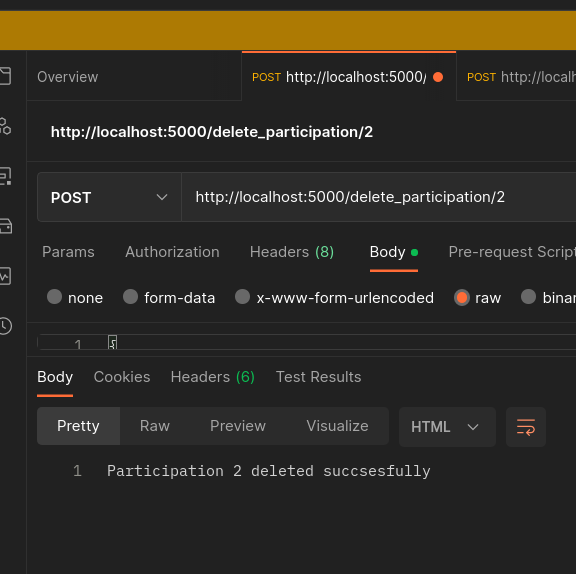
\includegraphics[scale=.5]{assets/participation/delete.png}
        \item Errores posibles: \begin{table}[H] \centering \begin{tabular}{|c|c|l|} \hline
        \textbf{Error Code} & \textbf{Description} \\ \hline \textit{400 Bad
        Request} & Algun identificador especificado no existe. \\ \hline
        \end{tabular} \end{table}
        
    \end{itemize}
\end{enumerate}

% schedule endpoints

\subsection{Schedule}
\begin{enumerate}
    \item \textbf{Crear Schedule}
    \begin{itemize}
        \item http://127.0.0.1:8002/Schedule/create\_schedule
        \item Donde va a crear un nuevo Schedule en la base de datos.
        \item Request y Response:
        \item 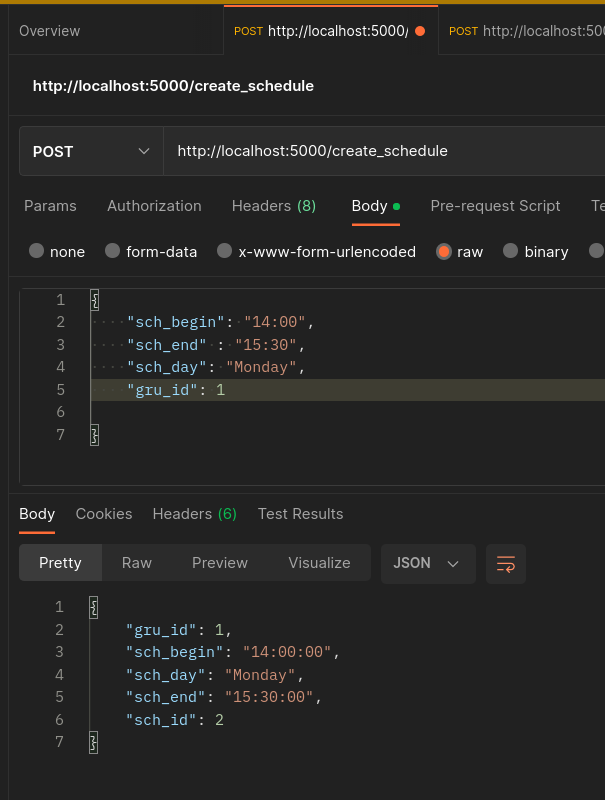
\includegraphics[scale=.5]{assets/schedule/create.png}
        \item Fields:
        \begin{table}[H] \centering \begin{tabular}{|l|l|l|l|} \hline
        \multicolumn{1}{|c|}{\textbf{Field}} &
        \multicolumn{1}{c|}{\textbf{Type}} &
        \multicolumn{1}{c|}{\textbf{Required?}} &
        \multicolumn{1}{c|}{\textbf{Description}} \\ \hline sch\_begin &
        datetime & required & La fecha y hora de inicio \\ \hline sch\_end &
        datetime & required & La fecha y hora del final \\ \hline sch\_day &
        varchar & required & El dia del Schedule \\ \hline gru\_id & int &
        required & El id del grupo que pertenece la Schedule \\ \hline
        \end{tabular} \end{table}
        \item Post objects:
        \begin{table}[H] \centering \begin{tabular}{|l|l|l|} \hline
        \multicolumn{1}{|c|}{\textbf{Field}} &
        \multicolumn{1}{c|}{\textbf{Type}} &
        \multicolumn{1}{c|}{\textbf{Description}} \\ \hline sch\_id & int & El
        identificador del Schedule \\ \hline sch\_begin & datetime & La fecha y
        hora de inicio \\ \hline sch\_end & datetime & La fecha y hora del final
        \\ \hline sch\_day & varchar & Una cadena de texto que representa el dia
        del Schedule \\ \hline gru\_id & int & Un identificador para cada grupo
        registrado \\ \hline \end{tabular} \end{table}

        \item Errores posibles: \begin{table}[H] \centering \begin{tabular}{|c|c|l|} \hline
        \textbf{Error Code} & \textbf{Description} \\ \hline \textit{400 Bad
        Request} & Algun identificador especificado no existe. \\ \hline
        \end{tabular} \end{table}
    \end{itemize}

    \item \textbf{Listar Schedule por ID}
    \begin{itemize}
        \item http://127.0.0.1:8002/Schedule/schedule/id
        \item Donde ``id'' es el identificador de la Schedule que se
        quiere especificar.
        \item Request y Response:
        \item 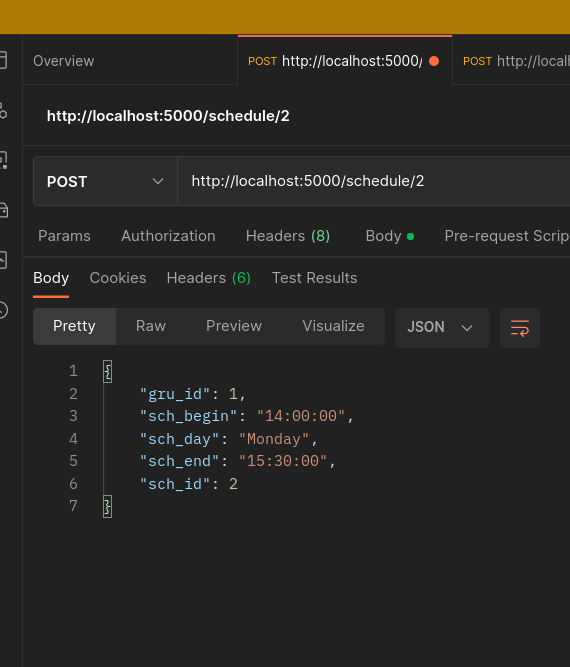
\includegraphics[scale=.5]{assets/schedule/schedule2.png}
        \item Post objects:
        \begin{table}[H] \centering \begin{tabular}{|l|l|l|} \hline
        \multicolumn{1}{|c|}{\textbf{Field}} &
        \multicolumn{1}{c|}{\textbf{Type}} &
        \multicolumn{1}{c|}{\textbf{Description}} \\ \hline sch\_id & int & El
        identificador del Schedule \\ \hline sch\_begin & datetime & La fecha y
        hora de inicio \\ \hline sch\_end & datetime & La fecha y hora del final
        \\ \hline sch\_day & varchar & Una cadena de texto que representa el dia
        del Schedule \\ \hline gru\_id & int & Un identificador para cada grupo
        registrado \\ \hline \end{tabular} \end{table}
        
        \item Errores posibles: \begin{table}[H] \centering \begin{tabular}{|c|c|l|}
        \hline \textbf{Error Code} & \textbf{Description} \\ \hline \textit{400
        Bad Request} & Algun identificador especificado no existe. \\ \hline
        \end{tabular} \end{table}
    \end{itemize}

    \item \textbf{Listar Schedule}
    \begin{itemize}
        \item http://127.0.0.1:8002/Schedule/schedules
        \item Donde se va a listar a todas las Schedules de la base de
        datos.
        \item Request y Response:
        \item 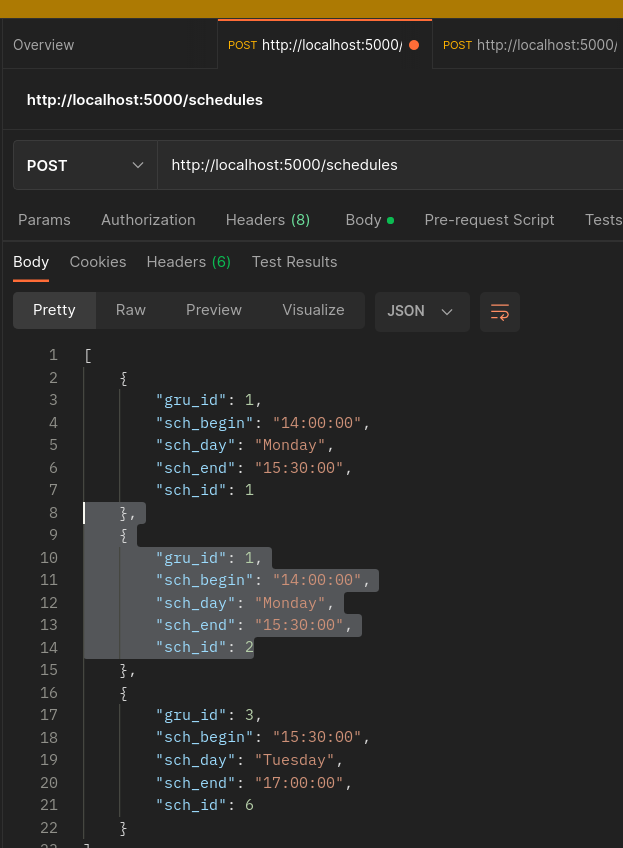
\includegraphics[scale=.5]{assets/schedule/schedules.png}
        \item Post Objects:
        \begin{table}[H] \centering \begin{tabular}{|l|l|l|} \hline
        \multicolumn{1}{|c|}{\textbf{Field}} &
        \multicolumn{1}{c|}{\textbf{Type}} &
        \multicolumn{1}{c|}{\textbf{Description}} \\ \hline sch\_id & int & El
        identificador del Schedule \\ \hline sch\_begin & datetime & La fecha y
        hora de inicio \\ \hline sch\_end & datetime & La fecha y hora del final
        \\ \hline sch\_day & varchar & Una cadena de texto que representa el dia
        del Schedule \\ \hline gru\_id & int & Un identificador para cada grupo
        registrado \\ \hline \end{tabular} \end{table}
    \end{itemize}

    \item \textbf{Actualizar Schedule}
    \begin{itemize}
        \item http://127.0.0.1:8002/Schedule/update\_schedule/id
        \item Donde se va a actualizar la Schedule del ID especificado.
        \item Request y Response:
        \item 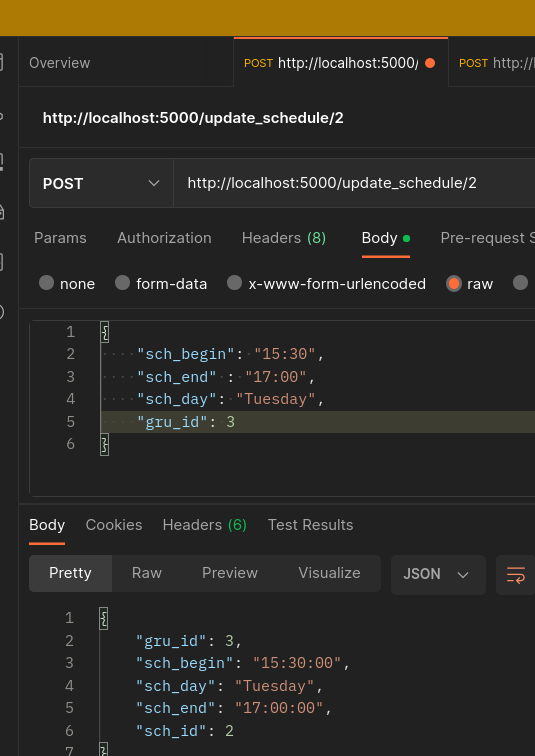
\includegraphics[scale=.5]{assets/schedule/update.png}
        \item Fields:
        \begin{table}[H] \centering \begin{tabular}{|l|l|l|l|} \hline
        \multicolumn{1}{|c|}{\textbf{Field}} &
        \multicolumn{1}{c|}{\textbf{Type}} &
        \multicolumn{1}{c|}{\textbf{Required?}} &
        \multicolumn{1}{c|}{\textbf{Description}} \\ \hline sch\_begin &
        datetime & required & La fecha y hora de inicio \\ \hline sch\_end &
        datetime & required & La fecha y hora del final \\ \hline sch\_day &
        varchar & required & El dia del Schedule \\ \hline gru\_id & int &
        required & El id del grupo que pertenece la Schedule \\ \hline
        \end{tabular} \end{table}
        \item Post objects:
        \begin{table}[H] \centering \begin{tabular}{|l|l|l|} \hline
        \multicolumn{1}{|c|}{\textbf{Field}} &
        \multicolumn{1}{c|}{\textbf{Type}} &
        \multicolumn{1}{c|}{\textbf{Description}} \\ \hline sch\_id & int & El
        identificador del Schedule \\ \hline sch\_begin & datetime & La fecha y
        hora de inicio \\ \hline sch\_end & datetime & La fecha y hora del final
        \\ \hline sch\_day & varchar & Una cadena de texto que representa el dia
        del Schedule \\ \hline gru\_id & int & Un identificador para cada grupo
        registrado \\ \hline \end{tabular} \end{table}

        \item Errores posibles: \begin{table}[H] \centering \begin{tabular}{|c|c|l|} \hline
        \textbf{Error Code} & \textbf{Description} \\ \hline \textit{400 Bad
        Request} & Algun identificador especificado no existe. \\ \hline
        \end{tabular} \end{table}
    \end{itemize}

    \item \textbf{Eliminar Schedule}
    \begin{itemize}
        \item http://127.0.0.1:8002/Schedule/delete\_schedule/id
        \item Donde se va a eliminar la Participation del ID especificado.
        \item Request y Response:
        \item 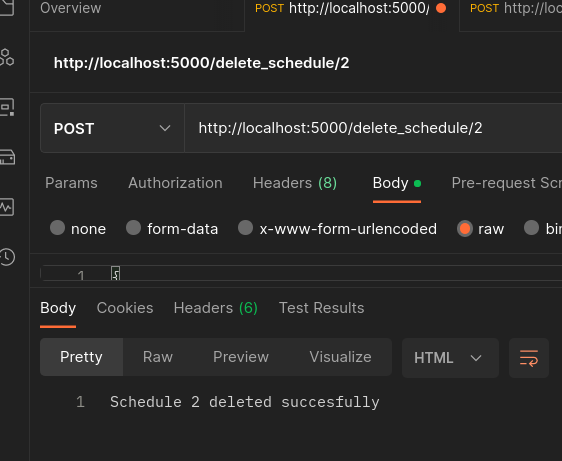
\includegraphics[scale=.5]{assets/schedule/delete.png}
        \item Errores posibles: \begin{table}[H] \centering
        \begin{tabular}{|c|c|l|} \hline \textbf{Error Code} &
        \textbf{Description} \\ \hline \textit{400 Bad Request} & Algun
        identificador especificado no existe. \\ \hline \end{tabular}
        \end{table}
    \end{itemize}
\end{enumerate}


% Student Endpoints 
\subsection{Student}
\begin{enumerate}
    \item \textbf{Crear Student}
    \begin{itemize}
        \item http://127.0.0.1:8002/Student/create\_student
        \item Donde va a crear un nuevo Student en la base de datos.
        \item Request y Response:
        \item 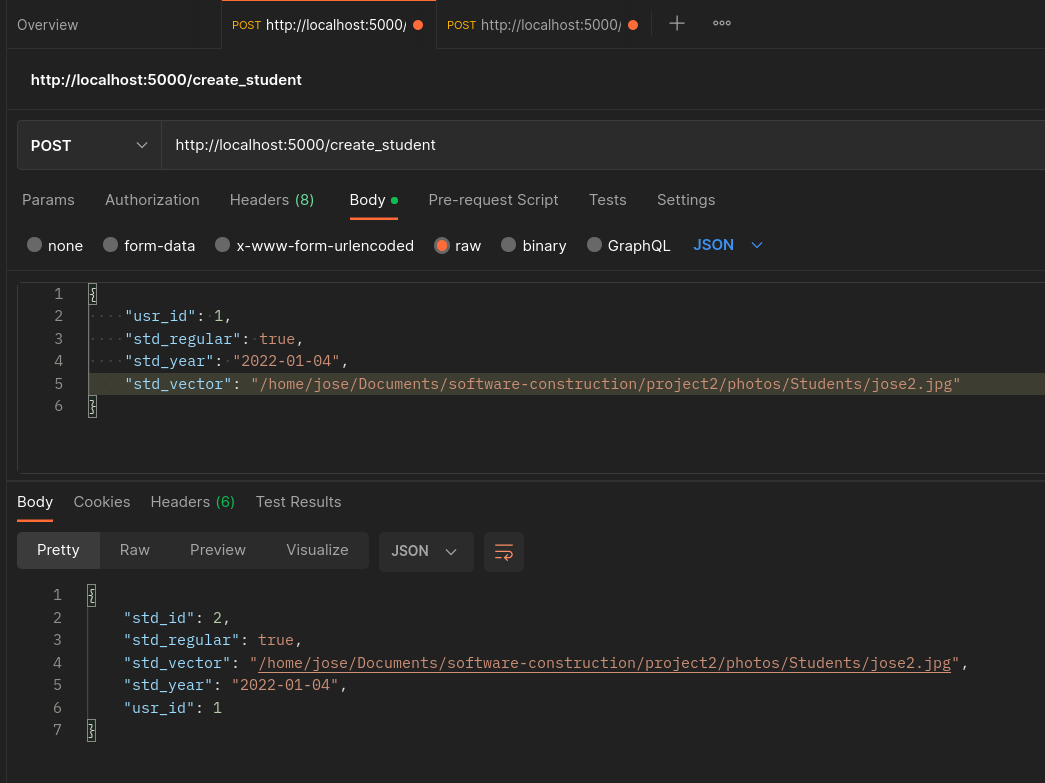
\includegraphics[scale=.5]{assets/student/create.png}
        \item Fields:
        \begin{table}[H] \centering \begin{tabular}{|l|l|l|l|} \hline
        \multicolumn{1}{|c|}{\textbf{Field}} &
        \multicolumn{1}{c|}{\textbf{Type}} &
        \multicolumn{1}{c|}{\textbf{Required?}} &
        \multicolumn{1}{c|}{\textbf{Description}} \\ \hline usr\_id & int &
        required & El identificador del User \\ \hline std\_regular & boolean &
        required & El tipo de matrícula que tiene. \\ \hline std\_year & date &
        required & Año en el que ingresó. \\ \hline \end{tabular} \end{table}
        \item Post objects:
        \begin{table}[H] \centering \begin{tabular}{|l|l|l|} \hline
        \multicolumn{1}{|c|}{\textbf{Field}} &
        \multicolumn{1}{c|}{\textbf{Type}} &
        \multicolumn{1}{c|}{\textbf{Description}} \\ \hline std\_id & int & El
        identificador del Student \\ \hline usr\_id & int & El identificador del
        User \\ \hline std\_regular & boolean & El tipo de matrícula que tiene.
        \\ \hline std\_year & date & Año en el que ingresó. \\ \hline
        \end{tabular} \end{table}
        \item Errores posibles: \begin{table}[H] \centering
        \begin{tabular}{|c|c|l|} \hline \textbf{Error Code} &
        \textbf{Description} \\ \hline \textit{400 Bad Request} & Algun
        identificador especificado no existe. \\ \hline \end{tabular}
        \end{table}
    \end{itemize}

    \item \textbf{Listar Student por ID}
    \begin{itemize}
        \item http://127.0.0.1:8002/Student/student/id
        \item Donde ``id'' es el identificador de la Student que se
        quiere especificar.
        \item Request y Response:
        \item 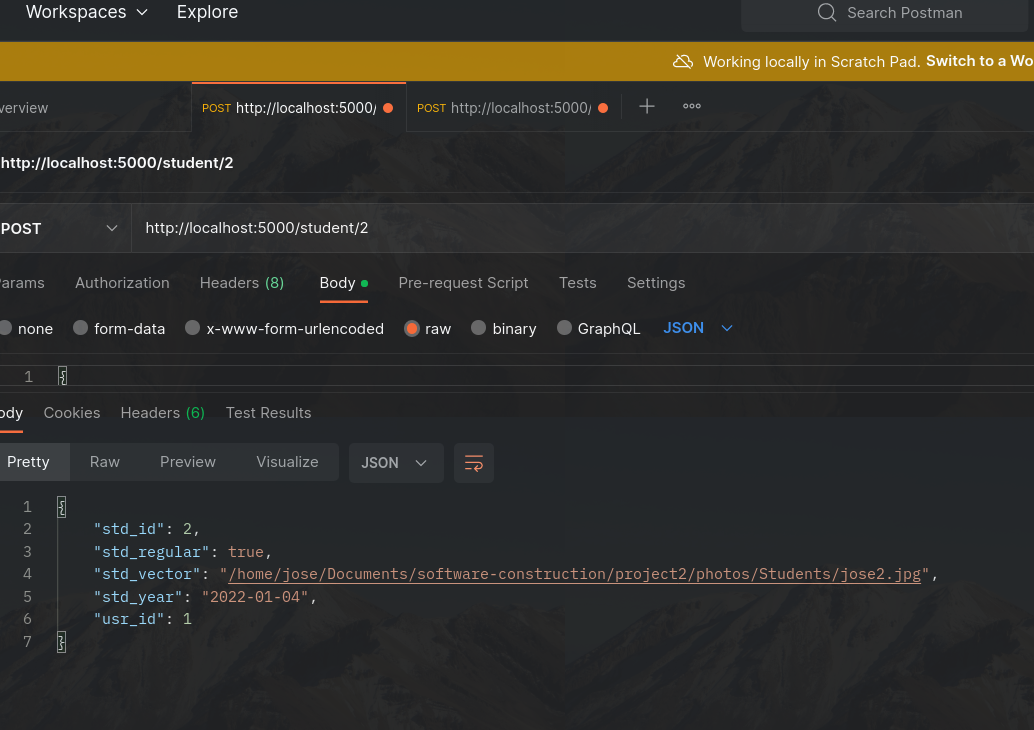
\includegraphics[scale=.5]{assets/student/student2.png}
        \item Post objects: \begin{table}[H] \centering \begin{tabular}{|l|l|l|}
        \hline \multicolumn{1}{|c|}{\textbf{Field}} &
        \multicolumn{1}{c|}{\textbf{Type}} &
        \multicolumn{1}{c|}{\textbf{Description}} \\ \hline std\_id & int & El
        identificador del Student \\ \hline usr\_id & int & El identificador del
        User \\ \hline std\_regular & boolean & El tipo de matrícula que tiene.
        \\ \hline std\_year & date & Año en el que ingresó. \\ \hline
        \end{tabular} \end{table} \item Errores posibles: \begin{table}[H] \centering
        \begin{tabular}{|c|c|l|} \hline \textbf{Error Code} &
        \textbf{Description} \\ \hline \textit{400 Bad Request} & Algun
        identificador especificado no existe. \\ \hline \end{tabular}
        \end{table}
    \end{itemize}

    \item \textbf{Listar Students}
    \begin{itemize}
        \item http://127.0.0.1:8002/Student/students
        \item Donde se va a listar a todas los Students de la base de
        datos.
        \item Request y Response:
        \item 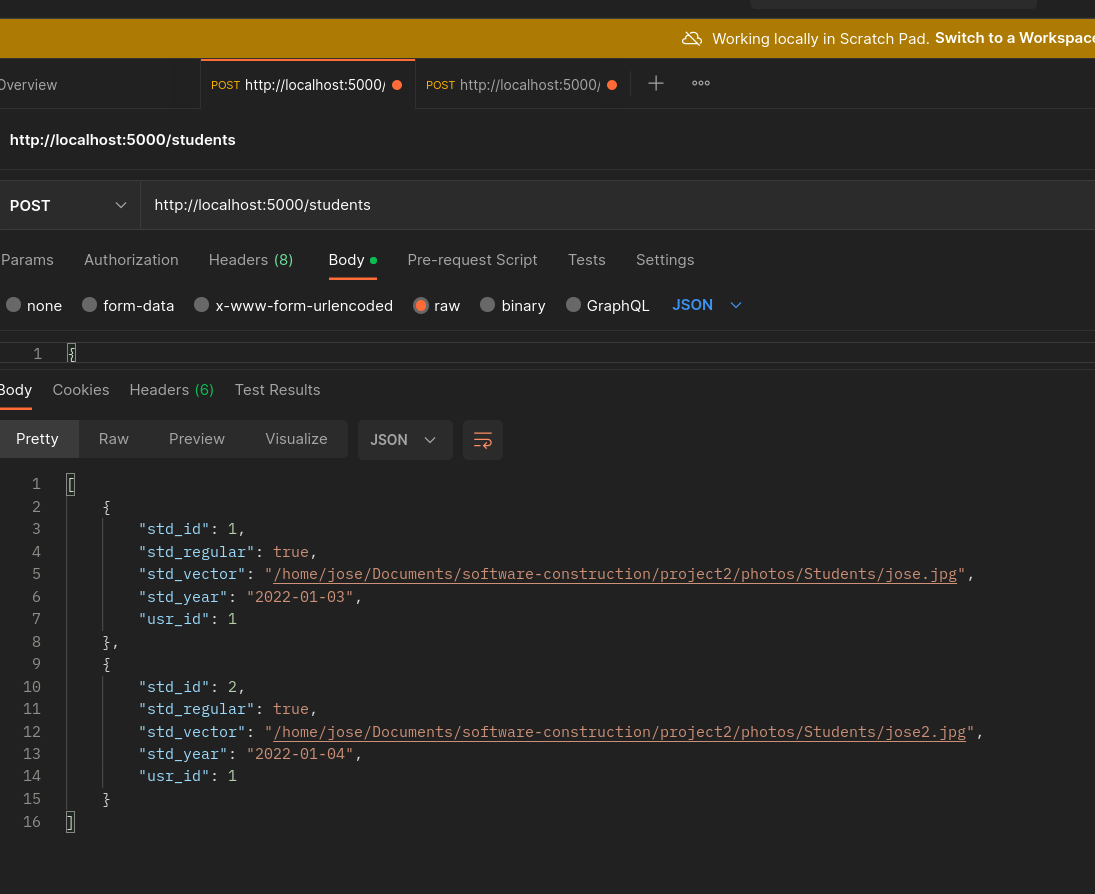
\includegraphics[scale=.5]{assets/student/students.png}
        \item Post objects: \begin{table}[H] \centering
        \begin{tabular}{|l|l|l|} \hline \multicolumn{1}{|c|}{\textbf{Field}} &
        \multicolumn{1}{c|}{\textbf{Type}} &
        \multicolumn{1}{c|}{\textbf{Description}} \\ \hline std\_id & int & El
        identificador del Student \\ \hline usr\_id & int & El identificador del
        User \\ \hline std\_regular & boolean & El tipo de matrícula que tiene.
        \\ \hline std\_year & date & Año en el que ingresó. \\ \hline
        \end{tabular} \end{table}
    \end{itemize}

    \item \textbf{Actualizar Student}
    \begin{itemize}
        \item http://127.0.0.1:8002/Student/update\_student/id
        \item Donde se va a actualizar la Student del ID especificado.
        \item Request y Response:
        \item 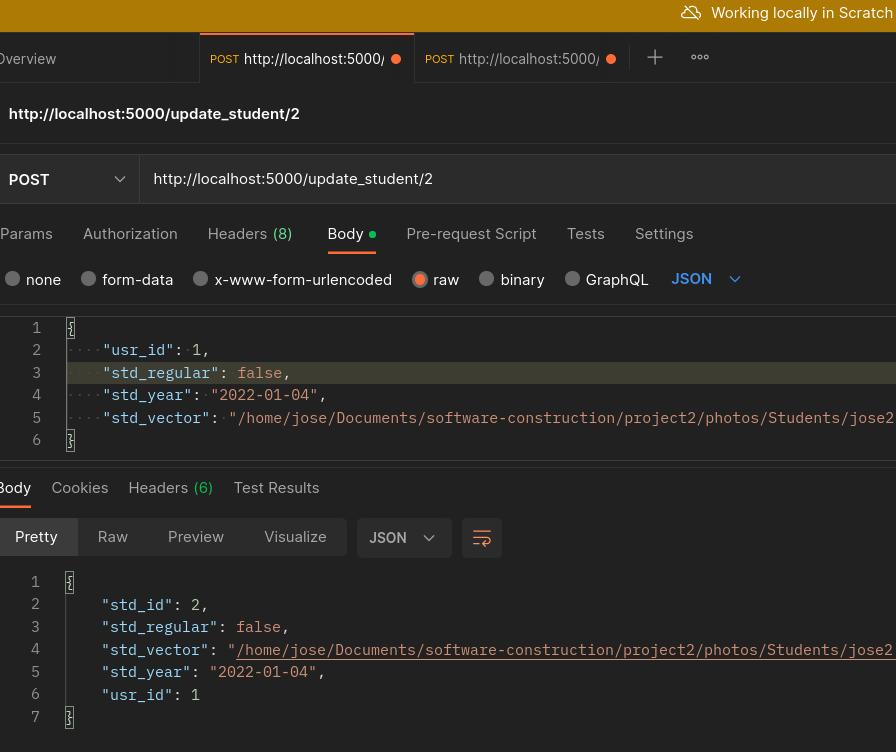
\includegraphics[scale=.5]{assets/student/update.png}
        \item Fields: \begin{table}[H] \centering \begin{tabular}{|l|l|l|l|} \hline
        \multicolumn{1}{|c|}{\textbf{Field}} &
        \multicolumn{1}{c|}{\textbf{Type}} &
        \multicolumn{1}{c|}{\textbf{Required?}} &
        \multicolumn{1}{c|}{\textbf{Description}} \\ \hline usr\_id & int &
        required & El identificador del User \\ \hline std\_regular & boolean &
        required & El tipo de matrícula que tiene. \\ \hline std\_year & date &
        required & Año en el que ingresó. \\ \hline \end{tabular} \end{table}
        \item Post objects: \begin{table}[H] \centering \begin{tabular}{|l|l|l|} \hline
        \multicolumn{1}{|c|}{\textbf{Field}} &
        \multicolumn{1}{c|}{\textbf{Type}} &
        \multicolumn{1}{c|}{\textbf{Description}} \\ \hline std\_id & int & El
        identificador del Student \\ \hline usr\_id & int & El identificador del
        User \\ \hline std\_regular & boolean & El tipo de matrícula que tiene.
        \\ \hline std\_year & date & Año en el que ingresó. \\ \hline
        \end{tabular} \end{table} \item Errores posibles: \begin{table}[H] \centering
        \begin{tabular}{|c|c|l|} \hline \textbf{Error Code} &
        \textbf{Description} \\ \hline \textit{400 Bad Request} & Algun
        identificador especificado no existe. \\ \hline \end{tabular}
        \end{table}
        
    \end{itemize}

    \item \textbf{Eliminar Student}
    \begin{itemize}
        \item http://127.0.0.1:8002/Student/delete\_student/id
        \item Donde se va a eliminar al Student del ID especificado.
        \item Request y Response:
        \item 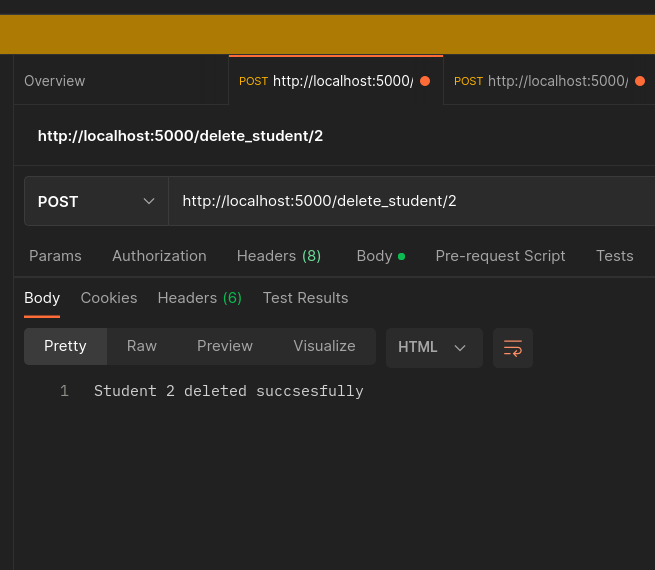
\includegraphics[scale=.5]{assets/student/delete.png}
        \item Errores posibles: \begin{table}[H] \centering
        \begin{tabular}{|c|c|l|} \hline \textbf{Error Code} &
        \textbf{Description} \\ \hline \textit{400 Bad Request} & Algun
        identificador especificado no existe. \\ \hline \end{tabular}
        \end{table}
    \end{itemize}
\end{enumerate}


 % teacher endpoints
\subsection{Teacher}
\begin{enumerate}
    \item \textbf{Crear Teacher}
    \begin{itemize}
        \item http://127.0.0.1:8002/Teacher/create\_teacher
        \item Donde va a crear un nuevo Teacher en la base de datos.
        \item Request y Response:
        \item 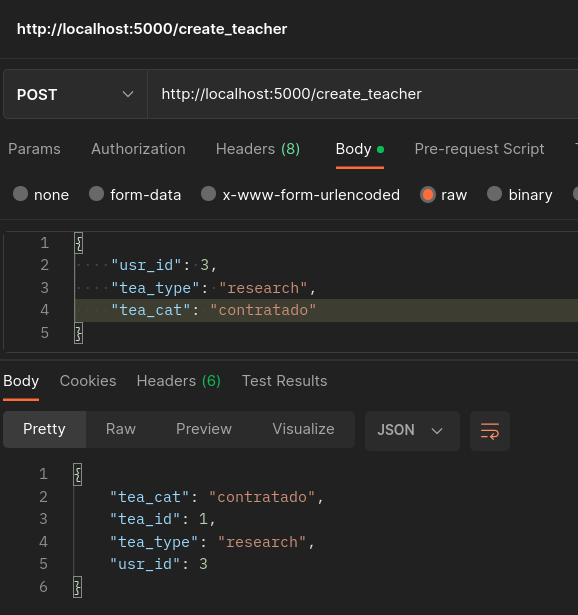
\includegraphics[scale=.5]{assets/teacher/create.png}
        \item Fields:
        \begin{table}[H] \centering \begin{tabular}{|l|l|l|l|} \hline
        \multicolumn{1}{|c|}{\textbf{Field}} &
        \multicolumn{1}{c|}{\textbf{Type}} &
        \multicolumn{1}{c|}{\textbf{Required?}} &
        \multicolumn{1}{c|}{\textbf{Description}} \\ \hline usr\_id & int &
        required & El identificador del User. \\ \hline tea\_type & varchar &
        required & El tipo de Teacher. \\ \hline tea\_cat & varchar & required &
        La categoría del Teacher. \\ \hline \end{tabular} \end{table}
        \item Post objects:
        \begin{table}[H] \centering \begin{tabular}{|l|l|l|} \hline
        \multicolumn{1}{|c|}{\textbf{Field}} &
        \multicolumn{1}{c|}{\textbf{Type}} &
        \multicolumn{1}{c|}{\textbf{Description}} \\ \hline tea\_id & int & El
        identificador del Teacher. \\ \hline usr\_id & int & El identificador
        del User. \\ \hline tea\_type & varchar & El tipo de Teacher. \\ \hline
        tea\_cat & varchar & La categoría del Teacher. \\ \hline \end{tabular}
        \end{table}
        \item Errores posibles: \begin{table}[H] \centering
        \begin{tabular}{|c|c|l|} \hline \textbf{Error Code} &
        \textbf{Description} \\ \hline \textit{400 Bad Request} & Algun
        identificador especificado no existe. \\ \hline \end{tabular}
        \end{table}
    \end{itemize}

    \item \textbf{Listar Teacher por ID}
    \begin{itemize}
        \item http://127.0.0.1:8002/Teacher/teacher/id
        \item Donde ``id'' es el identificador del Teacher que se quiere
        especificar.
        \item Request y Response:
        \item 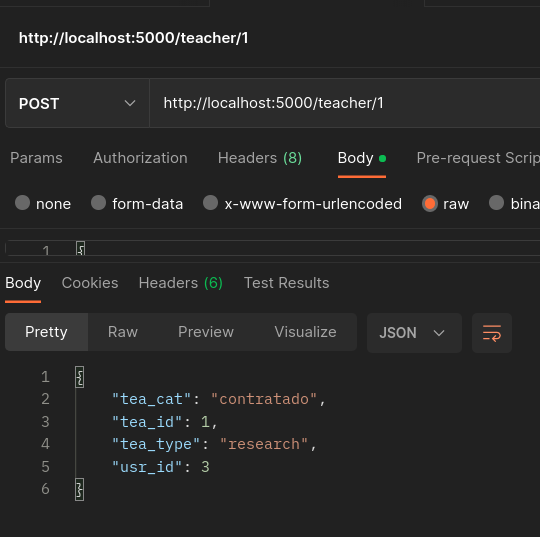
\includegraphics[scale=.5]{assets/teacher/teacher1.png}
        \item Post objects: \begin{table}[H] \centering \begin{tabular}{|l|l|l|}
        \hline \multicolumn{1}{|c|}{\textbf{Field}} &
        \multicolumn{1}{c|}{\textbf{Type}} &
        \multicolumn{1}{c|}{\textbf{Description}} \\ \hline tea\_id & int & El
        identificador del Teacher. \\ \hline usr\_id & int & El identificador
        del User. \\ \hline tea\_type & varchar & El tipo de Teacher. \\ \hline
        tea\_cat & varchar & La categoría del Teacher. \\ \hline \end{tabular}
        \end{table}
        
        \item Errores posibles: \begin{table}[H] \centering
        \begin{tabular}{|c|c|l|} \hline \textbf{Error Code} &
        \textbf{Description} \\ \hline \textit{400 Bad Request} & Algun
        identificador especificado no existe. \\ \hline \end{tabular}
        \end{table} 
    \end{itemize}

    \item \textbf{Listar Teacher por User ID}
    \begin{itemize}
        \item http://127.0.0.1:8002/Teacher/teachers
        \item Donde se va a listar a todos los Teachers de la base de
        datos.
        \item Request y Response:
        \item 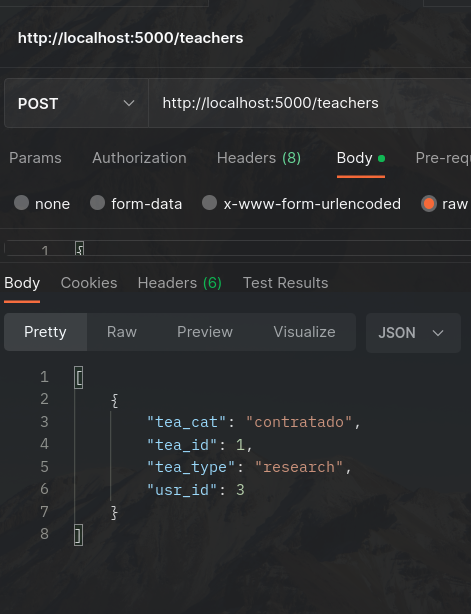
\includegraphics[scale=.5]{assets/teacher/teachers.png}
        \item Post objects: \begin{table}[H] \centering \begin{tabular}{|l|l|l|}
        \hline \multicolumn{1}{|c|}{\textbf{Field}} &
        \multicolumn{1}{c|}{\textbf{Type}} &
        \multicolumn{1}{c|}{\textbf{Description}} \\ \hline tea\_id & int & El
        identificador del Teacher. \\ \hline usr\_id & int & El identificador
        del User. \\ \hline tea\_type & varchar & El tipo de Teacher. \\ \hline
        tea\_cat & varchar & La categoría del Teacher. \\ \hline \end{tabular}
        \end{table}
    \end{itemize}

    \item \textbf{Actualizar Teacher}
    \begin{itemize}
        \item http://127.0.0.1:8002/Teacher/update\_teacher/id
        \item Donde se va a actualizar al Teacher del ID especificado.
        \item Request y Response:
        \item 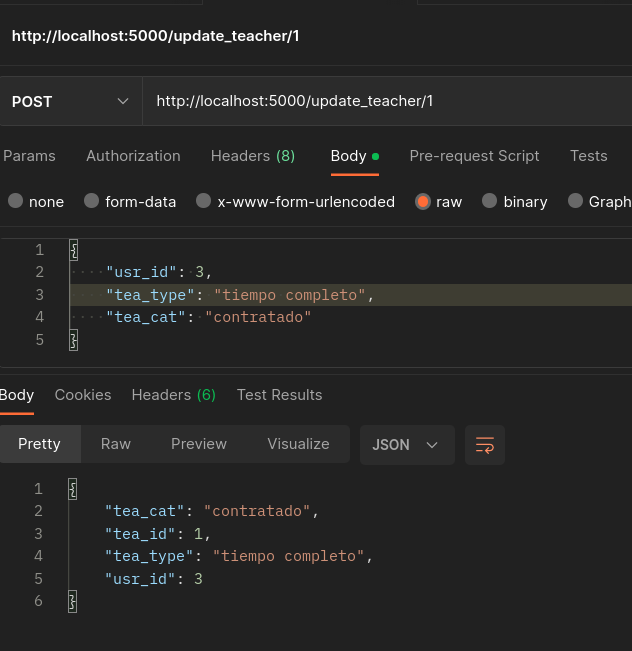
\includegraphics[scale=.5]{assets/teacher/update.png}
        \item Fields: \begin{table}[H] \centering \begin{tabular}{|l|l|l|l|} \hline
        \multicolumn{1}{|c|}{\textbf{Field}} &
        \multicolumn{1}{c|}{\textbf{Type}} &
        \multicolumn{1}{c|}{\textbf{Required?}} &
        \multicolumn{1}{c|}{\textbf{Description}} \\ \hline usr\_id & int &
        required & El identificador del User. \\ \hline tea\_type & varchar &
        required & El tipo de Teacher. \\ \hline tea\_cat & varchar & required &
        La categoría del Teacher. \\ \hline \end{tabular} \end{table} \item Post
        objects: \begin{table}[H] \centering \begin{tabular}{|l|l|l|} \hline
        \multicolumn{1}{|c|}{\textbf{Field}} &
        \multicolumn{1}{c|}{\textbf{Type}} &
        \multicolumn{1}{c|}{\textbf{Description}} \\ \hline tea\_id & int & El
        identificador del Teacher. \\ \hline usr\_id & int & El identificador
        del User. \\ \hline tea\_type & varchar & El tipo de Teacher. \\ \hline
        tea\_cat & varchar & La categoría del Teacher. \\ \hline \end{tabular}
        \end{table} \item Errores posibles: \begin{table}[H] \centering
        \begin{tabular}{|c|c|l|} \hline \textbf{Error Code} &
        \textbf{Description} \\ \hline \textit{400 Bad Request} & Algun
        identificador especificado no existe. \\ \hline \end{tabular}
        \end{table}
    \end{itemize}

    \item \textbf{Eliminar Teacher}
    \begin{itemize}
        \item http://127.0.0.1:8002/Teacher/delete\_teacher/id
        \item Donde se va a eliminar al Teacher del ID especificado.
        \item Request y Response:
        \item 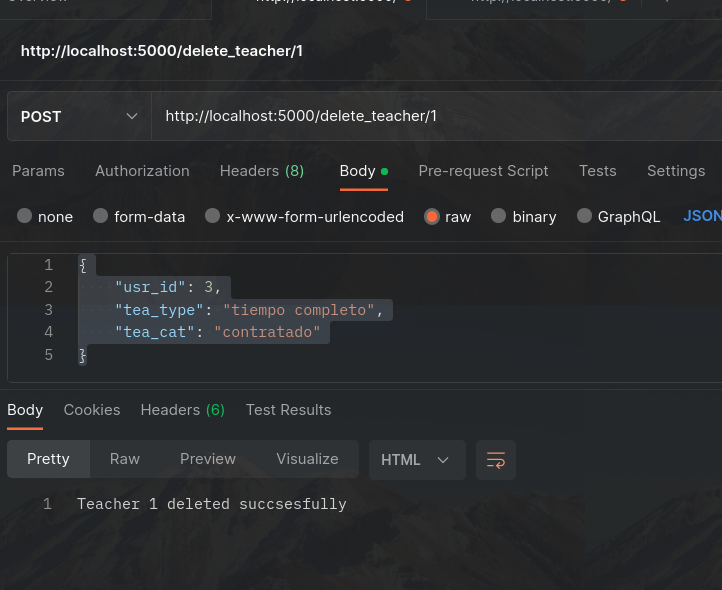
\includegraphics[scale=.5]{assets/teacher/delete.png}
        \item Errores posibles: \begin{table}[H] \centering
        \begin{tabular}{|c|c|l|} \hline \textbf{Error Code} &
        \textbf{Description} \\ \hline \textit{400 Bad Request} & Algun
        identificador especificado no existe. \\ \hline \end{tabular}
        \end{table}
    \end{itemize}
\end{enumerate}

% User Enpoint

\subsection{User}
\begin{enumerate}
    \item \textbf{Crear User}
    \begin{itemize}
        \item http://127.0.0.1:8002/User/create\_user
        \item Donde va a crear un nuevo User en la base de datos.
        \item Request y Response:
        \item 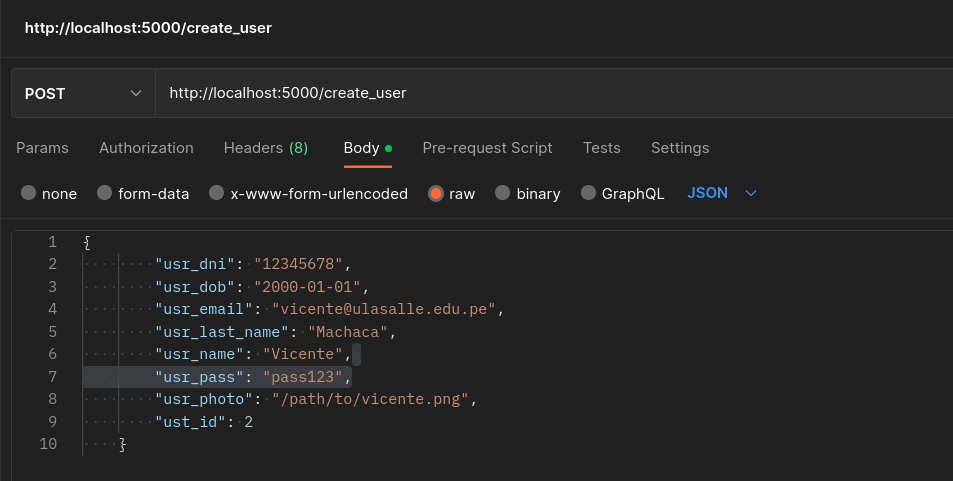
\includegraphics[scale=.5]{assets/user/create_user.png}
        \item Fields:
        \begin{table}[H] \centering \begin{tabular}{|l|l|l|l|} \hline
        \multicolumn{1}{|c|}{\textbf{Field}} &
        \multicolumn{1}{c|}{\textbf{Type}} &
        \multicolumn{1}{c|}{\textbf{Required?}} &
        \multicolumn{1}{c|}{\textbf{Description}} \\ \hline usr\_dni & varchar &
        required & El dni del User. \\ \hline usr\_pass & timestamp & required &
        La contraseña del User. \\ \hline usr\_photo & int & required & La foto
        del User. \\ \hline usr\_name & varchar & required & El nombre del User.
        \\ \hline usr\_last\_name & varchar & required & El apellido del User.
        \\ \hline usr\_dob & date & required & La fecha de nacimiento del User.
        \\ \hline usr\_email & varchar & required & El correo o email del User.
        \\ \hline ust\_id & int & required & El identificador del User\_type. \\
        \hline \end{tabular} \end{table}
        \item Post objects:
        \begin{table}[H] \centering \begin{tabular}{|l|l|l|} \hline
        \multicolumn{1}{|c|}{\textbf{Field}} &
        \multicolumn{1}{c|}{\textbf{Type}} &
        \multicolumn{1}{c|}{\textbf{Description}} \\ \hline usr\_id & int & El
        identificador del User. \\ \hline usr\_dni & varchar & El dni del User.
        \\ \hline usr\_pass & timestamp & La contraseña del User. \\ \hline
        usr\_photo & int & La foto del User. \\ \hline usr\_name & varchar & El
        nombre del User. \\ \hline usr\_last\_name & varchar & El apellido del
        User. \\ \hline usr\_dob & date & La fecha de nacimiento del User. \\
        \hline usr\_email & varchar & El correo o email del User. \\ \hline
        ust\_id & int & El identificador del User\_type. \\ \hline \end{tabular}
        \end{table}
        \item Errores posibles: \begin{table}[H] \centering
        \begin{tabular}{|c|c|l|} \hline \textbf{Error Code} &
        \textbf{Description} \\ \hline \textit{400 Bad Request} & Algun
        identificador especificado no existe. \\ \hline \end{tabular}
        \end{table}
    \end{itemize}

    \item \textbf{Listar User por ID}
    \begin{itemize}
        \item http://127.0.0.1:8002/User/user/id
        \item Donde ``id'' es el identificador de la User que se quiere especificar.
        \item Request y Response:
        \item 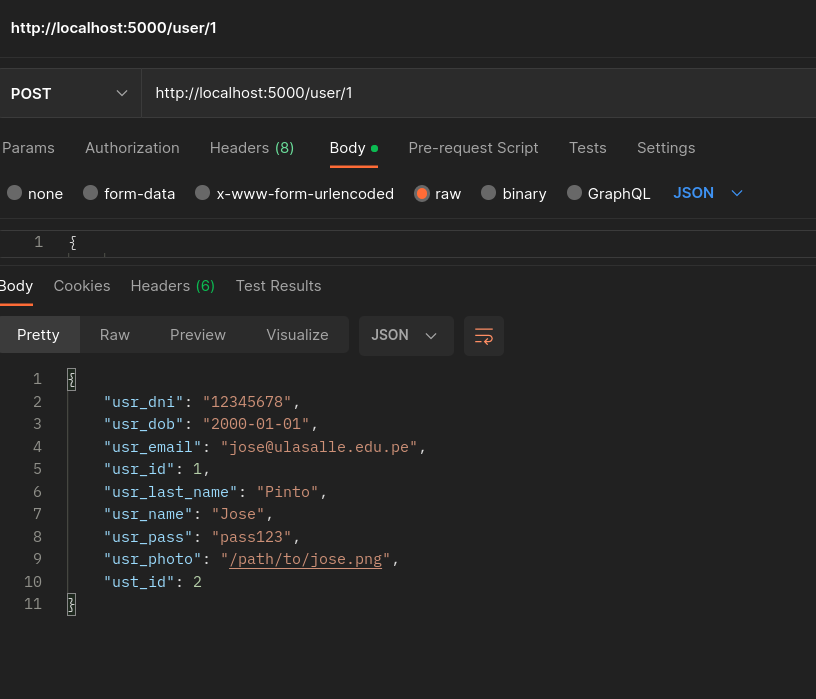
\includegraphics[scale=.5]{assets/user/user1.png}
        \item Post objects: \begin{table}[H] \centering \begin{tabular}{|l|l|l|}
        \hline \multicolumn{1}{|c|}{\textbf{Field}} &
        \multicolumn{1}{c|}{\textbf{Type}} &
        \multicolumn{1}{c|}{\textbf{Description}} \\ \hline usr\_id & int & El
        identificador del User. \\ \hline usr\_dni & varchar & El dni del User.
        \\ \hline usr\_pass & timestamp & La contraseña del User. \\ \hline
        usr\_photo & int & La foto del User. \\ \hline usr\_name & varchar & El
        nombre del User. \\ \hline usr\_last\_name & varchar & El apellido del
        User. \\ \hline usr\_dob & date & La fecha de nacimiento del User. \\
        \hline usr\_email & varchar & El correo o email del User. \\ \hline
        ust\_id & int & El identificador del User\_type. \\ \hline \end{tabular}
        \end{table} \item Errores posibles: \begin{table}[H] \centering
        \begin{tabular}{|c|c|l|} \hline \textbf{Error Code} &
        \textbf{Description} \\ \hline \textit{400 Bad Request} & Algun
        identificador especificado no existe. \\ \hline \end{tabular}
        \end{table}
    \end{itemize}

    \item \textbf{Listar User}
    \begin{itemize}
        \item http://127.0.0.1:8002/User/users
        \item Donde se va a listar a todas los Users de la base de datos.
        \item Request y Response:
        \item 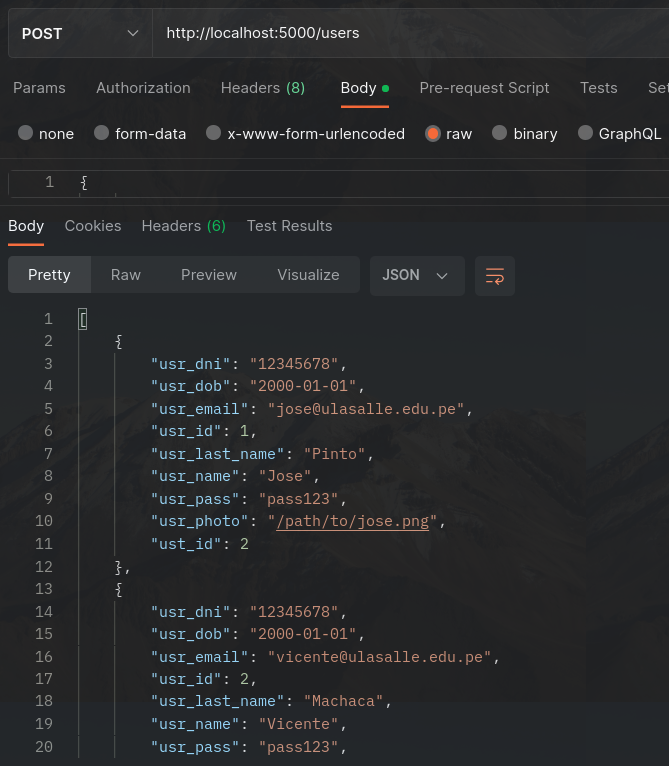
\includegraphics[scale=.5]{assets/user/users.png}
        \item Post objects: \begin{table}[H] \centering \begin{tabular}{|l|l|l|}
        \hline \multicolumn{1}{|c|}{\textbf{Field}} &
        \multicolumn{1}{c|}{\textbf{Type}} &
        \multicolumn{1}{c|}{\textbf{Description}} \\ \hline usr\_id & int & El
        identificador del User. \\ \hline usr\_dni & varchar & El dni del User.
        \\ \hline usr\_pass & timestamp & La contraseña del User. \\ \hline
        usr\_photo & int & La foto del User. \\ \hline usr\_name & varchar & El
        nombre del User. \\ \hline usr\_last\_name & varchar & El apellido del
        User. \\ \hline usr\_dob & date & La fecha de nacimiento del User. \\
        \hline usr\_email & varchar & El correo o email del User. \\ \hline
        ust\_id & int & El identificador del User\_type. \\ \hline \end{tabular}
        \end{table}
    \end{itemize}

    \item \textbf{Actualizar User}
    \begin{itemize}
        \item http://127.0.0.1:8002/User/update\_user/id
        \item Donde se va a actualizar la User del ID especificado.
        \item Request y Response:
        \item 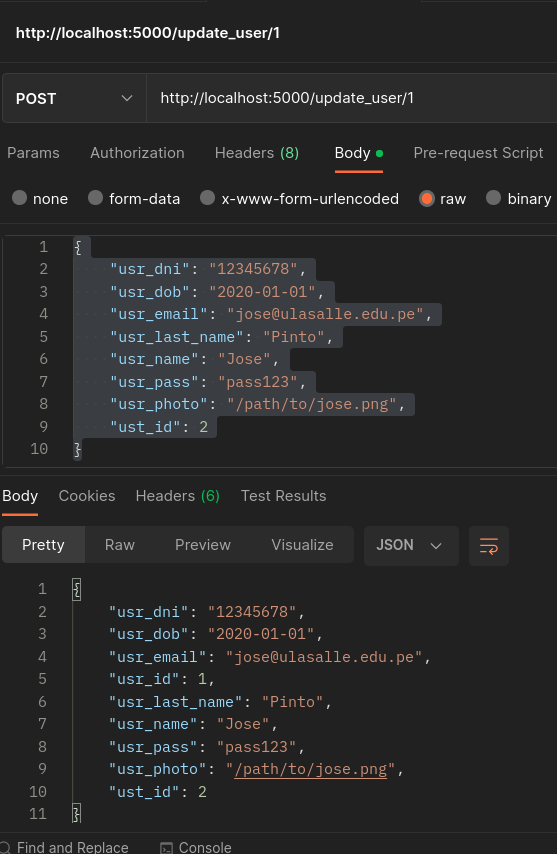
\includegraphics[scale=.5]{assets/user/update_user.png}
        \item Fields: \begin{table}[H] \centering \begin{tabular}{|l|l|l|l|} \hline
        \multicolumn{1}{|c|}{\textbf{Field}} &
        \multicolumn{1}{c|}{\textbf{Type}} &
        \multicolumn{1}{c|}{\textbf{Required?}} &
        \multicolumn{1}{c|}{\textbf{Description}} \\ \hline usr\_dni & varchar &
        required & El dni del User. \\ \hline usr\_pass & timestamp & required &
        La contraseña del User. \\ \hline usr\_photo & int & required & La foto
        del User. \\ \hline usr\_name & varchar & required & El nombre del User.
        \\ \hline usr\_last\_name & varchar & required & El apellido del User.
        \\ \hline usr\_dob & date & required & La fecha de nacimiento del User.
        \\ \hline usr\_email & varchar & required & El correo o email del User.
        \\ \hline ust\_id & int & required & El identificador del User\_type. \\
        \hline \end{tabular} \end{table} \item Post objects: \begin{table}[H] \centering
        \begin{tabular}{|l|l|l|} \hline \multicolumn{1}{|c|}{\textbf{Field}} &
        \multicolumn{1}{c|}{\textbf{Type}} &
        \multicolumn{1}{c|}{\textbf{Description}} \\ \hline usr\_id & int & El
        identificador del User. \\ \hline usr\_dni & varchar & El dni del User.
        \\ \hline usr\_pass & timestamp & La contraseña del User. \\ \hline
        usr\_photo & int & La foto del User. \\ \hline usr\_name & varchar & El
        nombre del User. \\ \hline usr\_last\_name & varchar & El apellido del
        User. \\ \hline usr\_dob & date & La fecha de nacimiento del User. \\
        \hline usr\_email & varchar & El correo o email del User. \\ \hline
        ust\_id & int & El identificador del User\_type. \\ \hline \end{tabular}
        \end{table} \item Errores posibles: \begin{table}[H] \centering
        \begin{tabular}{|c|c|l|} \hline \textbf{Error Code} &
        \textbf{Description} \\ \hline \textit{400 Bad Request} & Algun
        identificador especificado no existe. \\ \hline \end{tabular}
        \end{table}
    \end{itemize}

    \item \textbf{Eliminar User}
    \begin{itemize}
        \item http://127.0.0.1:8002/User/delete\_user/id
        \item Donde se va a eliminar al User del ID especificado.
        \item Request y Response:
        \item 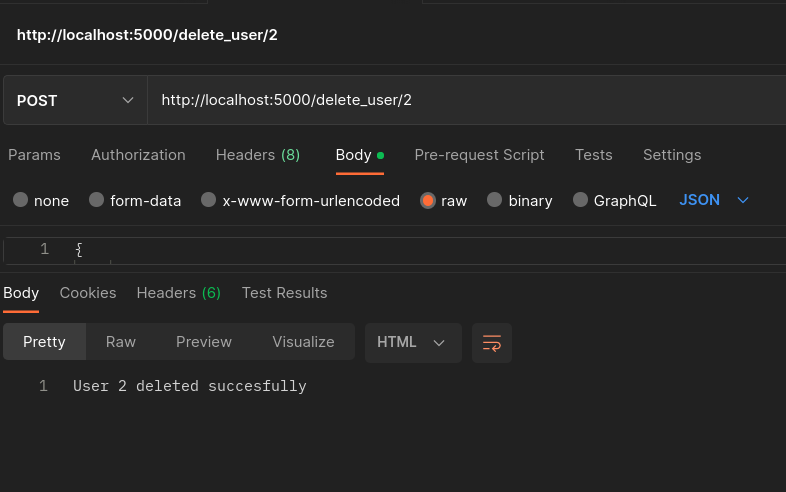
\includegraphics[scale=.5]{assets/user/delete_user.png}
        \item Errores posibles: \begin{table}[H] \centering
        \begin{tabular}{|c|c|l|} \hline \textbf{Error Code} &
        \textbf{Description} \\ \hline \textit{400 Bad Request} & Algun
        identificador especificado no existe. \\ \hline \end{tabular}
        \end{table}
    \end{itemize}
\end{enumerate}

% User_type endpoints

\subsection{User\_Type}
\begin{enumerate}
    \item \textbf{Crear User\_Type}
    \begin{itemize}
        \item http://127.0.0.1:8002/User\_type/create\_user\_type
        \item Donde va a crear un nuevo User\_type en la base de datos.
        \item Request y Response:
        \item 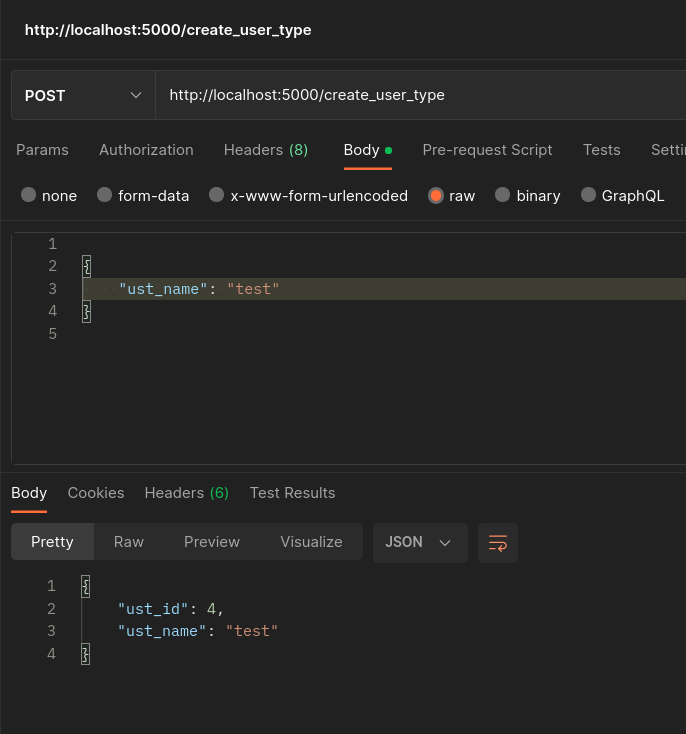
\includegraphics[scale=.5]{assets/user_type/create_user_type.png}
        \item Fields:
        \begin{table}[H] \centering \begin{tabular}{|l|l|l|l|} \hline
        \multicolumn{1}{|c|}{\textbf{Field}} &
        \multicolumn{1}{c|}{\textbf{Type}} &
        \multicolumn{1}{c|}{\textbf{Required}} &
        \multicolumn{1}{c|}{\textbf{Description}} \\ \hline ust\_name & varchar
        & required & El nombre del User\_type. \\ \hline \end{tabular}
        \end{table}
        Post Objects:
        \begin{table}[H] \centering \begin{tabular}{|l|l|l|} \hline
        \multicolumn{1}{|c|}{\textbf{Field}} &
        \multicolumn{1}{c|}{\textbf{Type}} &
        \multicolumn{1}{c|}{\textbf{Description}} \\ \hline ust\_id & int & El
        identificador del User\_type. \\ \hline ust\_name & varchar & El nombre
        del User\_type. \\ \hline \end{tabular} \end{table}
        \item Errores posibles: \begin{table}[H] \centering
        \begin{tabular}{|c|c|l|} \hline \textbf{Error Code} &
        \textbf{Description} \\ \hline \textit{400 Bad Request} & Algun
        identificador especificado no existe. \\ \hline \end{tabular}
        \end{table}
    \end{itemize}

    \item \textbf{Listar User\_type por ID}
    \begin{itemize}
        \item http://127.0.0.1:8002/User\_type/user\_type/id
        \item Donde ``id'' es el identificador del User\_type que se
        quiere especificar.
        \item Request y Response:
        \item 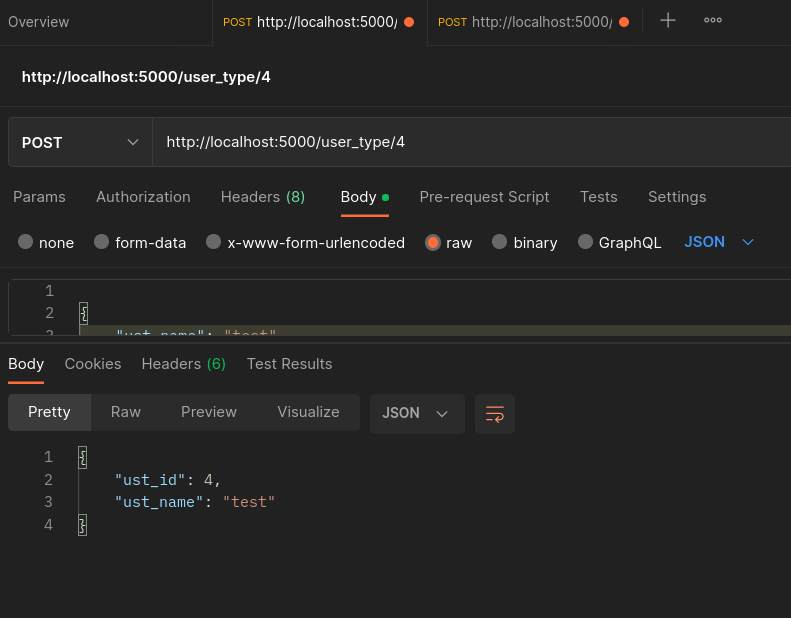
\includegraphics[scale=.5]{assets/user_type/user_type4.png}
        \item Post objects:
        Post Objects: \begin{table}[H] \centering \begin{tabular}{|l|l|l|} \hline
        \multicolumn{1}{|c|}{\textbf{Field}} &
        \multicolumn{1}{c|}{\textbf{Type}} &
        \multicolumn{1}{c|}{\textbf{Description}} \\ \hline ust\_id & int & El
        identificador del User\_type. \\ \hline ust\_name & varchar & El nombre
        del User\_type. \\ \hline \end{tabular} \end{table}
        \item Errores posibles: \begin{table}[H] \centering
        \begin{tabular}{|c|c|l|} \hline \textbf{Error Code} &
        \textbf{Description} \\ \hline \textit{400 Bad Request} & Algun
        identificador especificado no existe. \\ \hline \end{tabular}
        \end{table}

    \end{itemize}

    \item \textbf{Listar User\_types}
    \begin{itemize}
        \item http://127.0.0.1:8002/User\_type/user\_types
        \item Donde se va a listar a todos los User\_types de la base de
        datos.
        \item Request y Response:
        \item 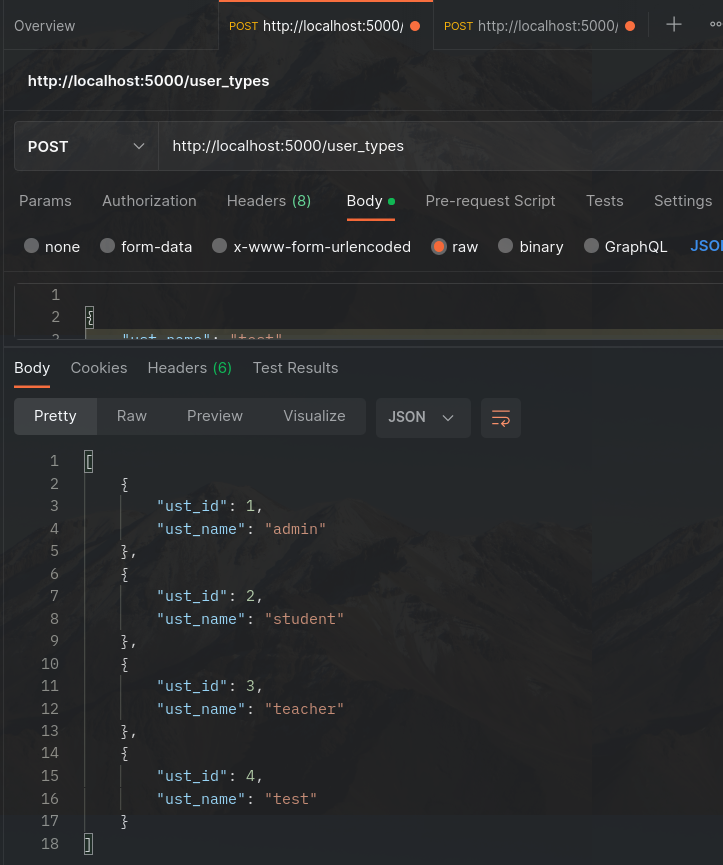
\includegraphics[scale=.5]{assets/user_type/user_types.png}
        \item Post objects: Post Objects: \begin{table}[H] \centering
        \begin{tabular}{|l|l|l|} \hline \multicolumn{1}{|c|}{\textbf{Field}} &
        \multicolumn{1}{c|}{\textbf{Type}} &
        \multicolumn{1}{c|}{\textbf{Description}} \\ \hline ust\_id & int & El
        identificador del User\_type. \\ \hline ust\_name & varchar & El nombre
        del User\_type. \\ \hline \end{tabular} \end{table}

    \end{itemize}

    \item \textbf{Actualizar User\_type}
    \begin{itemize}
        \item http://127.0.0.1:8002/User\_type/update\_user\_type/id
        \item Donde se va a actualizar al User\_type del ID especificado.
        \item Request y Response:
        \item \includegraphics[scale=.5]{assets/user_type/update_user_type.png}
        \item Fields:
        \begin{table}[H] \centering \begin{tabular}{|l|l|l|l|} \hline
        \multicolumn{1}{|c|}{\textbf{Field}} &
        \multicolumn{1}{c|}{\textbf{Type}} &
        \multicolumn{1}{c|}{\textbf{Required}} &
        \multicolumn{1}{c|}{\textbf{Description}} \\ \hline ust\_name & varchar
        & required & El nombre del User\_type. \\ \hline \end{tabular}
        \end{table} Post Objects: \begin{table}[H] \centering \begin{tabular}{|l|l|l|}
        \hline \multicolumn{1}{|c|}{\textbf{Field}} &
        \multicolumn{1}{c|}{\textbf{Type}} &
        \multicolumn{1}{c|}{\textbf{Description}} \\ \hline ust\_id & int & El
        identificador del User\_type. \\ \hline ust\_name & varchar & El nombre
        del User\_type. \\ \hline \end{tabular} \end{table} \item Errores
        posibles: \begin{table}[H] \centering \begin{tabular}{|c|c|l|} \hline \textbf{Error
        Code} & \textbf{Description} \\ \hline \textit{400 Bad Request} & Algun
        identificador especificado no existe. \\ \hline \end{tabular}
        \end{table}
    \end{itemize}

    \item \textbf{Eliminar User\_type}
    \begin{itemize}
        \item http://127.0.0.1:8002/User\_type/delete\_user\_type/id
        \item Donde se va a eliminar al User type del ID especificado.
        \item Request y Response:
        \item \includegraphics[scale=.5]{assets/user_type/delete_user_type.png}
        \item Errores posibles: \begin{table}[H] \centering
        \begin{tabular}{|c|c|l|} \hline \textbf{Error Code} &
        \textbf{Description} \\ \hline \textit{400 Bad Request} & Algun
        identificador especificado no existe. \\ \hline \end{tabular}
        \end{table}
    \end{itemize}
\end{enumerate}

%\clearpage
%\bibliographystyle{apalike}
\bibliographystyle{IEEEtranN}
\nocite{*}
\bibliography{refs.bib}
%\bibliography{bibliography}

\section{Repositorio}\label{sec:Repositorio}
\begin{itemize}
    \item {\color{blue}\href{https://github.com/pintovillamar/software-construction/tree/main/project2}{Parcial 1}}
\end{itemize}


\end{document}